

\section{Introduction}

\subsection{Installation}

This guide will go through the steps of installing ELMFIRE to a linux system. Windows users can use ELMFIRE by using a WSL installation, allowing the use of a linux subsystem within windows. More details on installing WSL can be found in https://www.geeksforgeeks.org/installation-guide/how-to-install-wsl2-windows-subsystem-for-linux-2-on-windows-10/ (make sure to stop at step 7, before the virtual machine section). This installation guide was tested on a clean install of Ubuntu 24.04

\textbf{Install Prerequisites:}

The following commands will install packages needed to build and run ELMFIRE:

\code{sudo apt-get update \&\& sudo apt-get upgrade -y}

\code{sudo apt-get install -y bc csvkit gdal-bin gfortran git jq libopenmpi-dev openmpi-bin pigz python3 python3-pip unzip wget zip}

Several Python libraries / packages, including three related to Google Remote Proecedure Call (gRPC), are needed to run the CloudFire microservices that provide ELMFIRE with fuel, weather, and ignition geospatial data. These can be installed system-wide as follows:

\code{sudo pip3 install google-api-python-client grpcio grpcio-tools python-dateutil --break-system-packages}

Alternatively, virtualenv can be used to prevent forcing a system-wide install as follows:

\code{sudo apt-get install python3-virtualenv}

\code{virtualenv \$HOME/virtualenv/elmfire}

\code{source \$HOME/virtualenv/elmfire/bin/activate/}

\code{\$HOME/virtualenv/elmfire/bin/pip3 install google-api-python-client grpcio grpcio-tools python-dateutil}

\textbf{Clone ELMFIRE Github repository:}

The current ELMFIRE repository can be cloned as follows:

\code{git clone https://github.com/lautenberger/elmfire.git}

Since this will clone the current repository, including all recent commits, for use in production environments a user may want to clone the latest stable release / branch instead, i.e.:

\code{git clone --branch 2025.1002 --single-branch https://github.com/lautenberger/elmfire.git}

\textbf{Set environment variables}

ELMFIRE uses four environment variables:

\begin{enumerate}
    \item \code{ELMFIRE\_SCRATCH\_BASE}: Full path to a scratch directory where the user has read/write access.
    \item \code{ELMFIRE\_BASE\_DIR}: Full path to the directory to which the ELMFIRE Git repository was cloned (i.e., the directory containing README.md).
    \item \code{ELMFIRE\_INSTALL\_DIR}: Full path to the directory where the ELMFIRE executable files will be installed (default: \$ELMFIRE\_BASE\_DIR/build/linux/bin).
    \item \code{CLOUDFIRE\\SERVER}: IP address of Cloudfire microservices server (this should be set to worldgen.cloudfire.io, more on this later).
\end{enumerate}

The easiest way to specify these variables is by exporting them from your \code{$\sim$/.bashrc} file. For example, one could pico \code{$\sim$/.bashrc} and then add the following lines (replacing /scratch/clauten, /home/clauten/elmfire, etc.):

\begin{verbatim}
export ELMFIRE_SCRATCH_BASE=/scratch/clauten
export ELMFIRE_BASE_DIR=/home/clauten/elmfire
export ELMFIRE_INSTALL_DIR=$ELMFIRE_BASE_DIR/build/linux/bin
export CLOUDFIRE_SERVER=worldgen.cloudfire.io
export PATH=$PATH:$ELMFIRE_INSTALL_DIR:$ELMFIRE_BASE_DIR/cloudfire
\end{verbatim}

These environment variables will be set on the next login or after sourcing the newly-edited file (\code{. $\sim$/.bashrc}).

\textbf{Build ELMFIRE executables:}

ELMFIRE and its postprocessing tool can be built as follows:

\begin{verbatim}
cd $ELMFIRE_BASE_DIR/build/linux
./make_gnu.sh
\end{verbatim}

Unless an error occurs, this will build the executables \code{elmfire\_VERSION} and \code{elmfire\_post\_VERSION} (where version is, for example, 2025.1002) and copy them to \code{\$ELMFIRE\_INSTALL\_DIR}. If this directory is not in the user’s \$PATH it should be added at this time. Note that two debug executables are also built.

At this point ELMFIRE has been installed in your local machine. Run the tutorial cases in \code{elmfire/tutorials/} to get started and verify everything was installed correctly.

\subsection{First Run}

ELMFIRE models the spread of a wildfire across a landscape and provides insightful outputs regarding the spread of the fire itself, the computation process or other post-processed results. The minimum information required to run an ELMFIRE simulation are:

\begin{itemize}
    \item Topography Rasters (Elevation, Slope, Aspect)
    \item Fuel Raster 
    \item Fuel Dictionary
    \item Canopy Values (Canopy Height, Canopy Base Height, Canopy Bulk Density, Canopy Cover)
    \item Ignition Location
    \item Transient Weather Values (Wind Magnitude, Wind Direction, 1-hour Fuel Moisture, 10-hour Fuel Moisture, 100-hour Fuel Moisture, Live Herbaceous Fuel Moisture, Live Woody Fuel moisture).
    \item Geospatial Domain Information (projection, cell size, lower-left X and Y coordinates).
\end{itemize}

The details of an ELMFIRE simulation, and the main way of using ELMFIRE, is through a .data text file, editable with a standard text editor program. For this guide, we will be naming this file elmfire.data . Below is the minimum required elmfire.data file to start an ELMFIRE simulation. Inputs are dictated through namelists (such as \&INPUTS) and inputs (such as \code{ASP\_FILENAME}). All inputs must be within their appropriate namelist. The order of inputs or namelists is not important. 

\begin{verbatim}
! Denotes a comment, everything after ! is ignored

!The inputs namelist contains parameters relating to parsing input data and setting 
!relevant parameters. *_DIRECTORY inputs denote parent folders, and *_FILENAME (for 
!weather, fuel and topography) refers to filename.tif. So, ASP_FILENAME = 'asp' means
!the aspect raster is /inputs/asp.tif.
&INPUTS     / Define all the input locations and parameters
FUELS_AND_TOPOGRAPHY_DIRECTORY = './inputs' 
ASP_FILENAME                   = 'asp'       
CBD_FILENAME                   = 'cbd'
CBH_FILENAME                   = 'cbh'
CC_FILENAME                    = 'cc'
CH_FILENAME                    = 'ch'
DEM_FILENAME                   = 'dem'
FBFM_FILENAME                  = 'fbfm13'
SLP_FILENAME                   = 'slp'
ADJ_FILENAME                   = 'adj'
PHI_FILENAME                   = 'phi'
WEATHER_DIRECTORY              = './inputs' 
WS_FILENAME                    = 'ws'
WD_FILENAME                    = 'wd'
M1_FILENAME                    = 'm1'
M10_FILENAME                   = 'm10'
M100_FILENAME                  = 'm100'
LH_MOISTURE_CONTENT            = 60
LW_MOISTURE_CONTENT            = 90
FOLIAR_MOISTURE_CONTENT        = 80
/

!The outputs namelist specifies details around the data and format that are going to
!be returned. In the example here, we only want the spread rate of the fire and the 
!time of arrival. All other outputs (other than general statistics) are assumed false.
&OUTPUTS
OUTPUTS_DIRECTORY    = './outputs'
DUMP_SPREAD_RATE     = .TRUE.
DUMP_TIME_OF_ARRIVAL = .TRUE.
CONVERT_TO_GEOTIFF   = .TRUE.
/

!The computational domain namelist sets parameters regarding the simulation space.
&COMPUTATIONAL_DOMAIN
A_SRS = 'EPSG: 32635'
COMPUTATIONAL_DOMAIN_CELLSIZE = 30
COMPUTATIONAL_DOMAIN_XLLCORNER = -1500
COMPUTATIONAL_DOMAIN_YLLCORNER = -1500
/

!The time control namelist dictates everything about the duration, step size and 
!temporal fidelity of the simulation. For now the only thing that needs to be specified
!is the duration of the simulation.
&TIME_CONTROL
SIMULATION_TSTOP = 36000
/

! The simulator namelist contains adjustment parameters, constants and other variables
!around the ELMFIRE solver itself. It is also where the ignition spots are specified. 
&SIMULATOR
NUM_IGNITIONS = 1
X_IGN(1)      = 0.0
Y_IGN(1)      = 3000.0
T_IGN(1)      = 3000.0
/

! The miscellaneous namelist contains other important parameters, most critically the
!path to GDAL in the user's computer, and a scratch directory for intermediate file 
!saves. 
&MISCELLANEOUS
PATH_TO_GDAL                   = '/usr/bin'
SCRATCH                        = './scratch'
/
\end{verbatim}

Then, this file is saved as elmfire.data in the same directory as the /inputs folder (containing out fuel, topography and weather information), the /scratch temporary file folder, and the /outputs folder. These folders are not automatically created by ELMFIRE and should be created by the user. 

Once all the files and folders are in place, the user can start ELMFIRE using the command (in a terminal in the main folder with the inputs/ , scratch/ and outputs/ folders):

\code{elmfire inputs/elmfire.data}

ELMFIRE will then start processing the input rasters, and then will run the main ELMFIRE routine. The expected output for the input file above would look like:

\begin{verbatim}
 ELMFIRE 2025.1002
 Reading &MISCELLANEOUS namelist group
 Reading &INPUTS namelist group
 Reading &OUTPUTS namelist group
 Reading &COMPUTATIONAL_DOMAIN namelist group
 Reading &TIME_CONTROL namelist group
 Reading &SIMULATOR namelist group
 Reading &WUI namelist group
 Reading &CALIBRATION namelist group
 Reading &SUPPRESSION namelist group
 Reading &SPOTTING namelist group
 Reading &SMOKE namelist group
 Reading &MONTE_CARLO namelist group
 Reading headers for fuels/topography and weather rasters
/usr/bin/gdal_translate -of ENVI -co "INTERLEAVE=BSQ" ./inputs/asp.tif ./scratch/asp.bsq
Input file size is 126, 126
0...10...20...30...40...50...60...70...80...90...100 - done.
/usr/bin/gdal_translate -of ENVI -co "INTERLEAVE=BSQ" ./inputs/ws.tif ./scratch/ws.bsq
Input file size is 126, 126
0...10...20...30...40...50...60...70...80...90...100 - done.
 Setting up shared memory, part 1
 Reading weather, fuel, and topography rasters
/usr/bin/gdal_translate -of ENVI -co "INTERLEAVE=BSQ" ./inputs/ws.tif ./scratch/ws.bsq
Input file size is 126, 126
0...10...20...30...40...50...60...70...80...90...100 - done.
/usr/bin/gdal_translate -of ENVI -co "INTERLEAVE=BSQ" ./inputs/wd.tif ./scratch/wd.bsq
Input file size is 126, 126
0...10...20...30...40...50...60...70...80...90...100 - done.
/usr/bin/gdal_translate -of ENVI -co "INTERLEAVE=BSQ" ./inputs/wd.tif ./scratch/wd.bsq
Input file size is 126, 126
0...10...20...30...40...50...60...70...80...90...100 - done.
/usr/bin/gdal_translate -of ENVI -co "INTERLEAVE=BSQ" ./inputs/m1.tif ./scratch/m1.bsq
Input file size is 126, 126
0...10...20...30...40...50...60...70...80...90...100 - done.
/usr/bin/gdal_translate -of ENVI -co "INTERLEAVE=BSQ" ./inputs/m1.tif ./scratch/m1.bsq
Input file size is 126, 126
0...10...20...30...40...50...60...70...80...90...100 - done.
/usr/bin/gdal_translate -of ENVI -co "INTERLEAVE=BSQ" ./inputs/m10.tif ./scratch/m10.bsq
Input file size is 126, 126
0...10...20...30...40...50...60...70...80...90...100 - done.
/usr/bin/gdal_translate -of ENVI -co "INTERLEAVE=BSQ" ./inputs/m10.tif ./scratch/m10.bsq
Input file size is 126, 126
0...10...20...30...40...50...60...70...80...90...100 - done.
/usr/bin/gdal_translate -of ENVI -co "INTERLEAVE=BSQ" ./inputs/m100.tif ./scratch/m100.bsq
Input file size is 126, 126
0...10...20...30...40...50...60...70...80...90...100 - done.
/usr/bin/gdal_translate -of ENVI -co "INTERLEAVE=BSQ" ./inputs/m100.tif ./scratch/m100.bsq
Input file size is 126, 126
0...10...20...30...40...50...60...70...80...90...100 - done.
 Reading fuel and topography rasters
/usr/bin/gdal_translate -of ENVI -co "INTERLEAVE=BSQ" ./inputs/asp.tif ./scratch/asp.bsq
Input file size is 126, 126
0...10...20...30...40...50...60...70...80...90...100 - done.
/usr/bin/gdal_translate -of ENVI -co "INTERLEAVE=BSQ" ./inputs/cbh.tif ./scratch/cbh.bsq
Input file size is 126, 126
0...10...20...30...40...50...60...70...80...90...100 - done.
/usr/bin/gdal_translate -of ENVI -co "INTERLEAVE=BSQ" ./inputs/cbh.tif ./scratch/cbh.bsq
Input file size is 126, 126
0...10...20...30...40...50...60...70...80...90...100 - done.
/usr/bin/gdal_translate -of ENVI -co "INTERLEAVE=BSQ" ./inputs/cbd.tif ./scratch/cbd.bsq
Input file size is 126, 126
0...10...20...30...40...50...60...70...80...90...100 - done.
/usr/bin/gdal_translate -of ENVI -co "INTERLEAVE=BSQ" ./inputs/cbd.tif ./scratch/cbd.bsq
Input file size is 126, 126
0...10...20...30...40...50...60...70...80...90...100 - done.
/usr/bin/gdal_translate -of ENVI -co "INTERLEAVE=BSQ" ./inputs/cc.tif ./scratch/cc.bsq
Input file size is 126, 126
0...10...20...30...40...50...60...70...80...90...100 - done.
/usr/bin/gdal_translate -of ENVI -co "INTERLEAVE=BSQ" ./inputs/cc.tif ./scratch/cc.bsq
Input file size is 126, 126
0...10...20...30...40...50...60...70...80...90...100 - done.
/usr/bin/gdal_translate -of ENVI -co "INTERLEAVE=BSQ" ./inputs/ch.tif ./scratch/ch.bsq
Input file size is 126, 126
0...10...20...30...40...50...60...70...80...90...100 - done.
/usr/bin/gdal_translate -of ENVI -co "INTERLEAVE=BSQ" ./inputs/ch.tif ./scratch/ch.bsq
Input file size is 126, 126
0...10...20...30...40...50...60...70...80...90...100 - done.
/usr/bin/gdal_translate -of ENVI -co "INTERLEAVE=BSQ" ./inputs/dem.tif ./scratch/dem.bsq
Input file size is 126, 126
0...10...20...30...40...50...60...70...80...90...100 - done.
/usr/bin/gdal_translate -of ENVI -co "INTERLEAVE=BSQ" ./inputs/dem.tif ./scratch/dem.bsq
Input file size is 126, 126
0...10...20...30...40...50...60...70...80...90...100 - done.
/usr/bin/gdal_translate -of ENVI -co "INTERLEAVE=BSQ" ./inputs/fbfm13.tif ./scratch/fbfm13.bsq
Input file size is 126, 126
0...10...20...30...40...50...60...70...80...90...100 - done.
/usr/bin/gdal_translate -of ENVI -co "INTERLEAVE=BSQ" ./inputs/fbfm13.tif ./scratch/fbfm13.bsq
Input file size is 126, 126
0...10...20...30...40...50...60...70...80...90...100 - done.
/usr/bin/gdal_translate -of ENVI -co "INTERLEAVE=BSQ" ./inputs/slp.tif ./scratch/slp.bsq
Input file size is 126, 126
0...10...20...30...40...50...60...70...80...90...100 - done.
/usr/bin/gdal_translate -of ENVI -co "INTERLEAVE=BSQ" ./inputs/slp.tif ./scratch/slp.bsq
Input file size is 126, 126
0...10...20...30...40...50...60...70...80...90...100 - done.
/usr/bin/gdal_translate -of ENVI -co "INTERLEAVE=BSQ" ./inputs/adj.tif ./scratch/adj.bsq
Input file size is 126, 126
0...10...20...30...40...50...60...70...80...90...100 - done.
/usr/bin/gdal_translate -of ENVI -co "INTERLEAVE=BSQ" ./inputs/adj.tif ./scratch/adj.bsq
Input file size is 126, 126
0...10...20...30...40...50...60...70...80...90...100 - done.
/usr/bin/gdal_translate -of ENVI -co "INTERLEAVE=BSQ" ./inputs/phi.tif ./scratch/phi.bsq
Input file size is 126, 126
0...10...20...30...40...50...60...70...80...90...100 - done.
/usr/bin/gdal_translate -of ENVI -co "INTERLEAVE=BSQ" ./inputs/phi.tif ./scratch/phi.bsq
Input file size is 126, 126
0...10...20...30...40...50...60...70...80...90...100 - done.
 Determining number of cases to run
 Allocating additional rasters
 Setting up shared memory, part 2
 Setting up statistics arrays
 ELMFIRE is running each ensemble member
 /usr/bin/gdal_translate -ot Float32 -co "COMPRESS=DEFLATE" -co "ZLEVEL=9" -a_srs "+proj=utm +zone=35 +datum=WGS84 +units=m +no_defs" ./scratch/vs_0000001_0259832.bil ./outputs/vs_0000001_0259832.tif
Input file size is 126, 126
0...10...20...30...40...50...60...70...80...90...100 - done.
/bin/rm -f ./scratch/vs_0000001_0259832.bil
/bin/rm -f ./scratch/vs_0000001_0259832.hdr
/usr/bin/gdal_translate -ot Float32 -co "COMPRESS=DEFLATE" -co "ZLEVEL=9" -a_srs "+proj=utm +zone=35 +datum=WGS84 +units=m +no_defs" ./scratch/time_of_arrival_0000001_0259832.bil ./outputs/time_of_arrival_0000001_0259832.tif
Input file size is 126, 126
0...10...20...30...40...50...60...70...80...90...100 - done.
/bin/rm -f ./scratch/time_of_arrival_0000001_0259832.bil
/bin/rm -f ./scratch/time_of_arrival_0000001_0259832.hdr
Meteorology band      1: Case #       1 complete.  Fire area:   3310.3 acres.
 End of simulation reached successfully. Shutting down.
\end{verbatim}
 
The above output shows an ELMFIRE simulation completed with no errors. Tutorial 1 contains a shell file that creates all the necessary files and folders for a simple simulation, and runs elmfire. 

The following sections will go into depth of the different variables, options and switches within ELMFIRE.

\section{Surface Fire Spread}
\label{surface_fire_spread}

Surface fire spread is the default fire spread mode of ELMFIRE, and will always run when the minimum inputs are provided. 

The first step in setting up ELMFIRE is to specify the geospatial input files. A distinction is made between weather files, and fuel and topography files. The fuel and topography files must be single-bad .tif files, all equal in extent and cellsize, colocated in space, and with a set NODATA value (even if none of the cells are NODATA). ELMFIRE does not check that these requirements are met and will crash with no relevant error message if any of these are not valid. The same goes with the variable type of each file.  Filenames should be specified without a suffix (e.g., 'slp', not 'slp.tif' because ELMFIRE automatically appends the .tif suffix to filenames (if they are virtual raster (.vrt) files, this behavior can be changed by setting VRT\_INSTEAD\_OF\_TIF = .TRUE.). The user must ensure that all GIS inputs are self-consistent.

The following landscape files are required:

\begin{enumerate}
    \item ASP\_FILENAME: Topographic aspect in degrees (16-bit integer)
    \item CBD\_FILENAME: Canopy bulk density in units of 100 kg per meter cubed (16-bit integer)
    \item CBH\_FILENAME: Canopy base height in units of 10 meters (16-bit integer)
    \item CC\_FILENAME: Canopy cover in units of percent (16-bit integer)
    \item CH\_FILENAME: Canopy height in units of 10 meters (16-bit integer)
    \item DEM\_FILENAME: Digital elevation model data in units of meters (16-bit integer)
    \item FBFM\_FILENAME: Fire behavior fuel model file (16-bit integer)
    \item SLP\_FILENAME: Topographic slope in degrees (16-bit integer)
    \item ADJ\_FILENAME: Surface spread rate adjustment factor (32-bit float)
    \item PHI\_FILENAME: Initial (level set variable) field (32-bit float)
\end{enumerate}

All of the above rasters, except for Phi and Adjustment, need to be Int16 variable data type. Phi and Adjustment must be Float32. The canopy parameters CBH and CH are in units of 10 meters, and CBD is in 100 kg per meter cubed. This is consistent with how these values are provided and reported in the US LANDFIRE database. If the input data of these files are in meters and kg per meter cubed respectively, the switches CBD\_TIMES\_100, CBH\_TIMES\_10 and CH\_TIMES\_10 can be set to .FALSE.. Note that the input rasters would then have to change change variable type from Int16 to Float32. Similarly, CC is read in percent as standard, but this can be changed by setting CC\_IN\_PERCENT to .FALSE.. Similar switches exist for DEAD\_MC\_IN\_PERCENT and LIVE\_MC\_IN\_PERCENT.

All the above is also true for the weather rasters, all of which need to be Float32. The weather values are specifically:

\begin{enumerate}
    \item WS\_FILENAME: 20-ft wind speed in mph
    \item WD\_FILENAME: 20-ft wind direction in degrees
    \item M1\_FILENAME: 1-hour dead fuel moisture content in %
    \item M10\_FILENAME: 10-hour dead fuel moisture content in %
    \item M100\_FILENAME: 100-hour dead fuel moisture content in %
\end{enumerate}

If the rasters specified above are single-band, then wind/weather conditions are assumed to be unchanging for the duration of the simulation. Transient wind/weather streams can be provided as input by using multi-band, or “stacked”, rasters. In that case, the parameter DT\_METEOROLOGY should be specified on the \&INPUT line. DT\_METEOROLOGY is the time interval (in seconds) between bands in the weather rasters. DT\_METEOROLOGY is commonly set to 3600 seconds due to the use of hourly reanalysis or forecast products to drive fire spread simulation. If wind speed is provided at 10 meters instead of 20 feet, the parameter WS\_AT\_10M should be set to .TRUE..

By default, live fuel moisture content (herbaceous, woody, and foliar) are spatially uniform and temporally unchanging. They are specified in the \&INPUTS namelist group via the keywords LH\_MOISTURE\_CONTENT, LW\_MOISTURE\_CONTENT, and FOLIAR\_MOISTURE\_CONTENT, respectively. Spatially varying live fuel moisture content can be specified by setting USE\_CONSTANT\_LH = .FALSE., USE\_CONSTANT\_LW = .FALSE., and USE\_CONSTANT\_FMC = .FALSE.. This directs ELMFIRE to read live fuel moisture from the rasters specified by MLH\_FILENAME, MLW\_FILENAME, FMC\_FILENAME (live herbaceous, live woody, and foliar, respectively). Even though live fuel moistures will typically change very little during a fire forecast (or hindcast), ELMFIRE expects the live fuel moisture rasters to have the same number of bands as the weather rasters, with the time interval between bands specified by DT\_METEOROLOGY.

ELMFIRE automatically interpolates between specific weather parameter steps, during the level set mode. The default behavior is a simple linear interpolation. Bilinear interpolation can also be used by turning WX\_BILINEAR\_INTERPOLATION = .TRUE. in the \&SIMULATOR namelist.

The Rothermel model requires midflame windspeed for its calculation. A wind adjustment factor is automatically calculated based on the algorithms in BEHAVE and Farsite. FARSITE and ELMFIRE assume a crown ratio of 1 for their calculation. This can be manually changed if needed through CROWN\_RATIO FPIXE:L. 


\subsection{Grid Declination}
\label{grid_declination}

In rare cases, direction rasters (specifically wind direction (WD) and aspect (ASP)) may have absolute north different from the absolute north of the domain. If this is the case, the difference between the true north of the simulation and the north of the wind direction and aspect measurements is called the grid declination. This can be accounted for in ELMFIRE, by setting the GRID\_DECLINATION float variable. Then the user should also set ROTATE\_WD to .TRUE. if the WD grid needs adjustment, and ROTATE\_ASP to .TRUE. if the Aspect grid needs adjustment.

\section{Computational domain size, extents, and resolution}
\label{computational_domain_size}

Input parameters controlling configuration of the computational domain are specified via the \&COMPUTATIONAL\_DOMAIN namelist group. The computational domain has the same extents of the input GIS fuels data, but its resolution can be the same or finer than the fuels inputs, meaning a computational domain with 10 m grid spacing can be used even if fuels inputs have a spatial resolution of 30 m.

The primary constraint is that the computational domain must fall completely within the GIS input data. This means that the computational domain can be the same size as or smaller than the input GIS data. Its spatial resolution can also be the same or finer than the input GIS fuels data.

The computational domain is specified by the following parameters:

\begin{itemize}
    \item A\_SRS: Projection of output files. Typically, a proj string would be used, i.e. A\_SRS = 'EPSG:32610'.
    \item COMPUTATIONAL\_DOMAIN\_CELLSIZE: spatial resolution of the computational domain, uniform in the x and y directions. This is commonly set to the spatial resolution of the input fuels layers (often 30 m) but can be set to a smaller value (e.g., 10 m) if a more highly resolved simulation is desired.
    \item COMPUTATIONAL\_DOMAIN\_XLLCORNER: x-coordinate of the lower left corner of the fuels inputs.
    \item COMPUTATIONAL\_DOMAIN\_YLLCORNER: y-coordinate of the lower left corner of the fuels inputs.
\end{itemize}

Note that this namelist group will soon be deleted since COMPUTATIONAL\_DOMAIN\_XLLCORNER, COMPUTATIONAL\_DOMAIN\_YLLCORNER, and A\_SRS can be determined internally from the fuels inputs’ metadata. When this happens, COMPUTATIONAL\_DOMAIN\_CELLSIZE will be moved to the \&SIMULATOR namelist group.

\section{Time}
\label{time}

Parameters related to time (simulation duration, computational timestep, etc.) are specified via the \&TIME\_CONTROL namelist group. A sample \&TIME\_CONTROL namelist group with key inputs is shown below:

\begin{verbatim}
&TIME_CONTROL
SIMULATION_TSTART   = 0.0
SIMULATION_TSTOP    = 3600.0
SIMULATION_DT       = 5.0
SIMULATION_DTMAX    = 600.0
TARGET_CFL          = 0.4
DT_INTERPOLATE_M1   = 300.0
DT_INTERPOLATE_M10  = 3000.0
DT_INTERPOLATE_M100 = 30000.0
DT_INTERPOLATE_MLH  = 9E8
DT_INTERPOLATE_MLW  = 9E8
DT_INTERPOLATE_FMC  = 9E8
DT_INTERPOLATE_WIND = 300.0
/
\end{verbatim}

Simulation start and stop times are specified via the keywords SIMULATION\_TSTART and SIMULATION\_TSTOP, respectively. These parameters have units of seconds, so a 12-hour simulation corresponds to SIMULATION\_TSTOP = 43200. The default value of SIMULATION\_TSTART is 0 seconds, meaning computations start at $t = 0$ seconds. This is generally appropriate for simulations driven by idealized or synthetic weather data. For transient wind/weather/fuel moisture multi-band rasters, Band 1 always corresponds to $t = 0$ seconds in ELMFIRE. The duration of an ELMFIRE simulation, while explicitly dictated, can be randomized between the start and stop times, through RANDOMIZE\_SIMULATION\_TSTOP.

When simulating real fires driven by transient, often hourly, weather streams it is usually desirable to start a fire spread simulation at a time > 0 seconds. Assuming that hourly weather fields are provided as input and fire’s time of ignition is 14:20, SIMULATION\_TSTART should be set to 1200.0, i.e., 20 minutes after the hour. In this particular case, Band 1 in all transient raster inputs should correspond to 14:00 and Band 2 should correspond to 15:00. The output files will contain rasters representing the unused weather bands, so some of the beginning or ending bands might be empty (or uniform). To crop the output rasters and only use the required weather bands, set ONLY\_READ\_NEEDED\_WX\_BANDS = .TRUE. in the \&INPUTS namelist.

The initial timestep is specified with the SIMULATION\_DT keyword. The timestep is automatically adjusted at runtime based on the Courant-Friedrichs-Lewy (CFL) conditions. The target CFL number can be specified by TARGET\_CFL. Since the internal timestep will change during a simulation, an upper limit on the allowable timestep can be specified with the SIMULATION\_DTMAX keyword.

Since wind/weather fields are often provided at hourly intervals but ELMFIRE’s computational timestep is usually on the order of a few to at most tens of seconds, ELMFIRE uses linear interpolation to determine wind/weather/fuel moisture conditions at intermediate times. This interpolation can be computationally expensive, so the user is provided with some control over the interpolation frequency. The keywords DT\_INTERPOLATE\_M1, DT\_INTERPOLATE\_M10, and DT\_INTERPOLATE\_M100 control the time between interpolations for 1-hour, 10-hour, and 100-hour fuel moistures. Wind speed and wind direction are controlled by DT\_INTERPOLATE\_WS and DT\_INTERPOLATE\_WD. As with other temporal inputs, units are seconds. The values quoted in the example \&TIME namelist above correspond to the standard values of ELMFIRE.

The start of each ELMFIRE simulation, or equivalently the specific hour of the first weather band, is assumed to be midnight. This can be changed (primarily for writing outputs) by changing the value of BAND\_ONE\_HOUR\_OF\_YEAR.

\subsection{Overnight Adjustment}
\label{overnight_adjustment}

The Rothermel model is well known to overpredict the rate of spread at night times, even when accounting for changes in dead fuel moisture content. ELMFIRE can account for this by multiplying its predicted rates of spread by an OVERNIGHT\_ADJUSTMENT\_FACTOR, set at 0.1 by default. This adjustment factor can be activated by setting USE\_DIURNAL\_ADJUSTMENT\_FACTOR to .TRUE.. ELMFIRE then internally estimates the sunset and sunrise hours, applying the diurnal adjustment factor between those two times. The parameters LATITUDE, LONGITUDE, CURRENT\_YEAR and HOUR\_OF\_YEAR should be set manually for this, as currently they are not inferred from any of the other input files. LATITUDE and LONGITUDE, CURRENT\_YEAR and HOUR\_OF\_YEAR should be set to reflect the rough center of the domain, the current year, and the elapsed hour within the year (so 2180 would refer to March 31st, 20:00) respectively. SUNRISE\_HOUR and SUNSET\_HOUR can be set directly if known.

With the above parameters, the sunrise and sunset times are known either by input or calculation. The start time of the simulation (note the difference between start time of simulation and ignition start time) can then be set by FORECAST\_START\_HOUR. 

Empirical evidence exists that dictates the main wildfire activity escalates some hours after sunrise and subsides some hours after sunset. To allow the user to include this observation to ELMFIRE, the overnight adjustment factor is not applied strictly between sunset and sunrise. Instead, the user must specify a BURN\_PERIOD\_LENGTH in hours for the total fire duration, and a BURN\_PERIOD\_CENTER\_FRAC, a fraction denoting whether the fire activity is concentrated in the early or late hours of the day. 

All the above is best explained with an example. Assume that for a specific fire the sunrise and sunset hours are 07:00 and 21:00 respectively. With a BURN\_PERIOD\_LENGTH of 12 hours, and a BURN\_PERIOD\_CENTER\_FRAC of 0.5, the mean hour of fire activity is $7+0.5\times (21-7)=14$. The diurnal adjustment factor then takes effect between $14 +0.5\times 12 = 20$ and $14-0.5\times 12 = 8$. Note how this result is antithetical to the initial empirical assumption this function was designed for. With a BURN\_PERIOD\_CENTER\_FRAC of 0.7, the mean hour of fire activity is $7+0.7\times (21-7)=16.8$. The diurnal adjustment factor then takes effect between $16.8 +0.5\times 12 = 22.8$ and $16.8-0.5\times 12 = 10.8$, which follows our observation. Expert judgement is required to fine tune these parameters for an accurate result. 


\section{Fire Initialization}

The two primary methods to initialize a fire spread simulation include point source ignitions and active fire perimeter initialization. These methods can be used concurrently, e.g. to simulate an active fire perimeter with additional point ignitions or spot fire initiation outside of the fire perimeter.

\subsection{Point source ignitions}
\label{point_source_ignitions}

One or more point source ignitions can be specified on the \&SIMULATOR namelist group via the keywords X\_IGN(:), Y\_IGN(:), and T\_IGN(:) which respectively control point ignitions’ x- and y-coordinates, and time of ignitions. As an example, the following lines specify two separate point source ignitions:

\begin{verbatim}
&SIMULATOR
NUM_IGNITIONS = 2
X_IGN(1)      = 1000.0
Y_IGN(1)      = 1000.0
T_IGN(1)      = 0.0
X_IGN(2)      = 2000.0
Y_IGN(2)      = 2000.0
T_IGN(2)      = 7200.0
\end{verbatim}

The first ignition occurs at (x,y) = (1000.0, 1000.0) at simulation time 0.0 seconds and the second occurs at (x,y) = (2000.0, 2000.0) at simulation time = 7200.0 seconds. The keyword NUM\_IGNITIONS specifies the total number of point source ignitions. Ignitions should be numbered sequentially starting at 1 and ending at NUM\_IGNITIONS. The number of point source ignitions is currently limited to 100.

\subsection{Active fire perimeters}

The fire front position is tracked by solving a conservation equation for the level set variable $\phi$ where unburned areas correspond to 
$\phi > 0$, burned areas correspond to 
$\phi < 0$, and the fire front position is the level set corresponding to 
$\phi = 0$. At the start of a simulation ELMFIRE reads the initial 
field from a 32-bit floating point raster with filename PHI\_FILENAME as specified in the \&INPUTS namelist group.

If there is no active fire at the start of a simulation, then all pixels in the PHI\_FILENAME raster should be initialized with a single start value greater than 0 (usually 1.0). An initial fire front position can be specified by burning a value less than 0 (usually -1.0) into the PHI\_FILENAME raster. All pixels with an initial 
value less than 0 will be marked as burned and fire spread will be initiated from those pixels.

Extinguished or “cold” segments of the fire perimeter can be simulated by modifying the fuel model raster to have a non-burnable fuel model in extinguished segments of the fire perimeter.

\section{Outputs}
\label{outputs}

A sample \&OUTPUTS namelist group is shown below:

\begin{verbatim}
&OUTPUTS
OUTPUTS_DIRECTORY         = './outputs'
DTDUMP                    = 3600.
DUMP_FLIN                 = .TRUE.
DUMP_SPREAD_RATE          = .TRUE.
DUMP_SURFACE_FIRE         = .TRUE.
DUMP_TIME_OF_ARRIVAL      = .TRUE.
/
\end{verbatim}

The keyword OUTPUTS\_DIRECTORY specifies the directory to which ELMFIRE will write its output files. This output directory must exist at run-time; it will not be automatically created. Transient outputs such as DUMP\_SURFACE\_FIRE will be dumped every DTDUMP seconds.

In general, outputs to be dumped are specified using a logical keyword that begins with DUMP\_*. The following is a full list of raster outputs and the logical keywords that control whether they are written to disk. 

Most output parameters are written as standard during or after an ELMFIRE simulation. These parameters are given below. Outputs could be rasters of CSV files, showing either the final parameters or transient steps through the simulation, with intervals dictated by DTDUMP.

\begin{cfTable}{The main dump routine outputs of ELMFIRE.}{tab:main_dump}{1.0\textwidth}
\begin{tabular}{lp{4cm}lll}
\specialrule{1.2pt}{0pt}{0pt}
\multicolumn{5}{c}{MAIN DUMP ROUTINE}                                                                                                 \\
Option                     & Description                                              & Units                    & Type   & Output    \\
\specialrule{1.2pt}{0pt}{0pt}
DUMP\_TRANSIENT\_ACREAGE   & Total fire scar size over time                           & acres                    & CSV    & Final     \\
DUMP\_SURFACE\_FIRE        & Status of surface fire (1 = burned, 0 = unburned)        & Categorical              & Raster & Transient \\
DUMP\_CROWN\_FIRE          & Status of crown fire (0 = none, 1 = passive, 2 = active) & Categorical              & Raster & Transient \\
DUMP\_CRITICAL\_FLIN       & Surface Fireline intensity required for crown fire ignition & kW/m                  & Raster & Final     \\
DUMP\_SPREAD\_RATE         & Rate of Spread Magnitude                                 & ft/min                   & Raster & Final     \\
DUMP\_SPREAD\_DIRECTION    & Rate of Spread Direction                                 & degrees                  & Raster & Final     \\
DUMP\_HPUA                 & Heat per unit area                                       & kJ/$m^2$                 & Raster & Final     \\
DUMP\_FLIN                 & Fireline Intensity                                       & kW/m                     & Raster & Final     \\
DUMP\_FLAME\_LENGTH        & Flame Length                                             & ft                       & Raster & Final     \\
DUMP\_REACTION\_INTENSITY  & Reaction intensity                                       & kW/$m^2$                 & Raster & Final     \\
DUMP\_WS20                 & Wind speed                                               &                          & Raster & Transient \\
DUMP\_WD20                 & Wind direction                                           & degrees                  & Raster & Transient \\
DUMP\_VELOCITY             & Rate of Spread                                           & ft/min                   & Raster & Final     \\
DUMP\_TIME\_OF\_ARRIVAL    & Fire arrival time                                        & s                        & Raster & Final     \\
DUMP\_TOTAL\_DFC\_RECEIVED & Accumulated heat flux due to direct flame contact (WU-E) & kJ/$m^2$                 & Raster & Final \\
DUMP\_TOTAL\_RAD\_RECEIVED & Accumulated heat flux due to radiation (WU-E)            & kJ/$m^2$                 & Raster & Final \\
DUMP\_TRANSIENT\_DFC         & Transient DFC heat flux (WU-E)                           & kW/$m^2$                 & Raster & Transient \\
DUMP\_TRANSIENT\_RAD         & Transient radiation heat flux (WU-E)                     & kW/$m^2$                 & Raster & Transient \\
DUMP\_HRR\_TRANSIENT       & Transient heat release rate per unit area                & kW/$m^2$                 & Raster & Transient \\
DUMP\_TAGGED               & Show currently 'Tagged' Cells (1 = Tagged)               & Categorical              & Raster & Transient \\
DUMP\_PHI                  & Level set phi variable                                   & -                        & Raster & Transient \\
DUMP\_EMBER\_FLUX          & Accumulated ember flux per Monte-Carlo ensemble          & pieces/$m^2$             & Raster & Final \\
DUMP\_EMBER\_FLUX\_TRANSIENT & Transient ember flux at the moment                     & pieces/$m^2$             & Raster & Transient  \\
DUMP\_SPOTTING\_OUTPUTS    & Ember spatial and temporal travel data                   & coordinates, s           & CSV    & Final    \\
\specialrule{1.2pt}{0pt}{0pt}
\end{tabular}
\end{cfTable}

Output filenames are hardcoded but should be readily discernable, e.g. fireline intensity outputs begin with flin\_, time of arrival outputs begin with toa\_, etc. Since ELMFIRE is sometimes used to run multiple cases as part of a Monte Carlo analysis or sensitivity analysis, a seven-digit sequential identifier is prepended to the name of each output raster, and the time at which the raster was dumped is appended to the filename.

If a monte carlo simulation set is done, especially with random or multiple ignitions, it is useful to plot the scalar outputs on a map, depending on their ignition locations. Each run can be given an initial RUN\_ID string, to differentiate it from potential other monte-carlo runs. The outputs that are possible in this case are:

\begin{cfTable}{The postprocessed output routine options of ELMFIRE.}{tab:postprocess}{1.0\textwidth}
\begin{tabular}{lp{6cm}l}
\multicolumn{3}{c}{POSTPROCESS}                                                                                           \\
Switch                              & Description                                                       & Units           \\
\specialrule{1.2pt}{0pt}{0pt}
CALCULATE\_TIMES\_BURNED            &                                                                   & sims            \\
CALCULATE\_FLAME\_LENGTH\_STATS     & Output maximum and average flame length                           & ft              \\
USE\_FLAME\_LENGTH\_BINS            & Split the flame length occurrence in bins                  & bin number      \\
USE\_EMBER\_COUNT\_BINS             & Split the firebrand count occurrence in bins                  & bin number      \\
DUMP\_SURFACE\_FIRE\_AREA           & Surface fire area occurring from each ignition spot                & acres           \\
DUMP\_CROWN\_FIRE\_AREA             & Crown fire area occurring from each ignition spot                  & acres           \\
DUMP\_FIRE\_VOLUME                  & Fire volume occurring from each ignition spot                      & ac-ft           \\
DUMP\_AFFECTED\_POPULATION          & Affected population occurring from each ignition spot              & input dependent \\
DUMP\_AFFECTED\_REAL\_ESTATE\_VALUE & Affected real estate value occurring from each ignition spot & input dependent \\
DUMP\_AFFECTED\_LAND\_VALUE         & Affected land value occurring from each ignition spot              & input dependent \\
DUMP\_EMBER\_FLUX                   & Ember flux occurring from each ignition spot                       &                 \\
ACCUMULATE\_EMBER\_FLUX             &                                                                   &                
\end{tabular}
\end{cfTable}

The flame length and ember count bins are specified manually. That is, following the example below (same for the FLAME parameters).

\begin{verbatim}
USE_EMBER_LENGTH_BINS = .TRUE.
NUM_EMBER_COUNT_BINS  = 3
EMBER_COUNT_BIN_LO(1) = 0
EMBER_COUNT_BIN_HI(1) = 10
EMBER_COUNT_BIN_LO(2) = 11
EMBER_COUNT_BIN_HI(2) = 25
EMBER_COUNT_BIN_LO(3) = 26
EMBER_COUNT_BIN_HI(3) = 50

\end{verbatim}

Some additional output switches that might work different from the ones listed above are:

\begin{itemize}
    \item TIME\_AT\_BURNED\_ACRES(:): Output the time (mins) and runtime (s) taken for the fire to reach some amount of acres. Multiple acre values can be tracked, by including, for example, TIME\_AT\_BURNED\_ACRES(1) = 500 and at another line TIME\_AT\_BURNED\_ACRES(2) = 1000.
    \item DUMP\_HOURLY\_RASTERS: 
    \item DUMP\_BINARY\_OUTPUTS: Save some outputs (ignition x, y) and additional parameters if FULL\_BINARY\_OUTPUTS = .TRUE. (time of arrival, flame length, velocity, crown fire) in binary format. Only for fire areas larger than MINIMUM\_AREA\_FOR\_BINARY\_OUTPUTS ( = 0 as standard). To save on space a limited, randomised percentage of timesteps can be written to the binary file by specifying a BINARY\_OUTPUTS\_DUMP\_FRACTION ( = 1.00 by default)
    \item DUMP\_SPOTTING\_IGNITION\_TIME: (deactivated)
    \item DUMP\_TIMINGS: Show individual processor timings
    \item If a TIMED\_LOCATIONS\_CSV file is provided in the \&INPUTS namelist, then for all points specified in the csv (rows of point ID, X dimension, Y dimension), the arrival time of the fire will be saved in a new TIMED\_LOCATION\_TRACKER\_1.csv.
\end{itemize}


ELMFIRE initially outputs all raster data as BIL rasters, a line-separated raster data type easy to use with FORTRAN. Then ELMFIRE converts these BIL rasters (along with their associated HDR header files) to geoTIFF files. In doing so, the BIL and HDR files are permanently deleted. This behavior can be changed by setting CONVERT\_TO\_GEOTIFF to .FALSE..

\subsection{Virtual Weather Stations}
\label{virtual_weather_stations}

Virtual weather stations can be specified by setting NUM\_VIRTUAL\_STATIONS to an integer greater than zero, and then specifying x and y coordinates of each station. As a simple example, data from two virtual stations would be written to disk by adding the following lines to the \&OUTPUTS namelist group:

\begin{verbatim}
NUM_VIRTUAL_STATIONS = 2
VIRTUAL_STATION_X(1) = 12345.0
VIRTUAL_STATION_Y(1) = 67890.0
VIRTUAL_STATION_X(2) = 98765.0
VIRTUAL_STATION_Y(2) = 43210.0
\end{verbatim}

The index inside the parentheses denotes the station number. For each virtual station a separate .csv file will be written that includes transient and fixed quantities as a function of time. These quantities are currently:

\begin{itemize}
    \item Elevation
    \item Slope
    \item Aspect
    \item Canopy Bulk Density
    \item Canopy Base Height
    \item Canopy Cover
    \item Canopy Height
    \item Fuel model
    \item 1-hour dead fuel moisture
    \item 10-hour dead fuel moisture
    \item 100-hour dead fuel moisture
    \item Live herbaceous fuel moisture
    \item Live woody fuel moisture
    \item Foliar fuel moisture
    \item 20-ft wind speed
    \item 20-ft wind direction
    \item Phi (level set variable)
\end{itemize}

Note that virtual stations have been temporarily \textbf{disabled}.

\section{Miscellaneous}
\label{misc}

Custom fuel models, of either vegetated or building fuels, can be specified by including related .csv files, following from fuel\_models.csv. The csv files contain a series of fuel parameters. The location of these files is in the folder MISCELLANEOUS\_INPUTS\_DIRECTORY, and named FUEL\_MODEL\_FILE.csv and BUILDING\_FUEL\_MODEL\_FILE.csv. The FUEL\_MODEL\_FILE.csv has the following structure:

\begin{verbatim}
1,FBFM01,.FALSE.,0.034,0,0,0,0,3500,9999,9999,1,12,8000
\end{verbatim}

Corresponding to:
\begin{itemize}
    \item Fuel Number: 1
    \item Fuel Name: FBFM01
    \item Dynamic Fuel: No
    \item 1h Fuel Load: 0.034 $lb\; ft^{-2}$
    \item 10h Duel Load: 0 $lb\; ft^{-2}$
    \item 100h Fuel Load: 0 $lb\; ft^{-2}$
    \item Live Herbaceous Fuel Load: 0 $lb\; ft^{-2}$
    \item Live woody Fuel Load: 0 $lb\; ft^{-2}$
    \item 1h Surface Area to Volume Ratio (SAV): 3500 $ft^2 ft^{-3}$
    \item Live and Dead Herbaceous SAV: 9999 $ft^2 ft^{-3}$
    \item Live Woody SAV: 9999 $ft^2 ft^{-3}$
    \item Fuel Load Depth: 1.0 ft
    \item Dead Fuel Moisture of Extinction: 12 \%
    \item Heat Content: 8000 $BTU\;lb^{-1}$
\end{itemize}

Hardcoded values within ELMFIRE are the same for all fuel models:

\begin{itemize}
    \item 10h SAV: 109 $ft^2 ft^{-3}$
    \item 100h SAV: 30 $ft^2 ft^{-3}$
    \item Particle Density: 32 $lb\;ft^{-3}$
    \item Total Mineral Content: 0.055
    \item Effective Mineral Content: 0.01
\end{itemize}

A building fuel model would look like:

\begin{verbatim}
1,ST01,300,400,10080,14400,360,25,10500,9,0.89,8,0.5,100,0.0,20
\end{verbatim}

Corresponding to:
\begin{itemize}
    \item Fuel Number: 1
    \item Fuel Name: ST01
    \item Time to HRR of 1 MW: 300 s
    \item HRR Rise Time: 400 s
    \item HRR Peak Time: 10080 s
    \item FRR Decay Time: 14400 s
    \item Fuel Load: 360
    \item Peak HRR Per Unit Area: 25
    \item Critical FTP: 10500
    \item Q Critical: 9
    \item Absorptivity: 0.89
    \item Building Height: 8 m
    \item Nonburnable fraction: 0.5
    \item Probability of ignition from firebrands: 100 \%
    \item Ember Ignition Hardening Factor: 0
    \item Time to ignition from Embers: 20 s
\end{itemize}


For temporary file storage and intermediate saves, ELMFIRE can use a scratch directory instead of the output directory. This folder can be specified using the SCRATCH variable. By default, this folder is used to store intermediate geospatial files. ELMFIRE converts the input geoTIFF files to binary, easier-to-process BSQ files. BSQ files come with associated XML or HDR files containing their metadata. If, for any reason, the BSQ files can be provided directly instead of the geoTIFF files (which would slightly speed up the initial data processing step), they can be used in ELMFIRE by setting USE\_EXISTING\_BSQS = .TRUE. in the \&INPUT namelist. ELMFIRE will then search for associated XML metadata files, but this can be switched to HDR files through USE\_BSQ\_XML\_HEADER = .FALSE..  

In some use cases of ELMFIRE, the fire domain may be split into multiple files. Specifically, there are cases where the ignition is within the landscape of one geotiff file, but the overall burn area is extended to eight additional, neighboring rasters. Should this be the case, USE\_TILED\_IO can be set to .TRUE., and ELMFIRE will combine the fire landscape from the eight input files. These files should be named, using aspect as an example, asp\_1\_2.tif, where 1 and 2 refer to the rasters position in space. In this case, this raster would be the top-middle part of the landscape. The files should range from asp\_1\_1.tif to asp\_3\_3.tif. 

The location that contains gdal functions and programs is assumed to be usr/bin/. If that is not the case, the location can be changed through PATH\_TO\_GDAL.

\section{Physics and Numerics options}

Runtime options are specified via the \&SIMULATOR namelist group. Brief descriptions of how various parameters influence physics options are presented below.

\subsection{Elliptical dimensions}
\label{elliptical_dimensions}

In ELMFIRE, every point along the fire front behaves as an independent elliptical wavelet (Huygens principle). However, since the underlying surface fire spread model only provides the rate of spread in the head fire direction, the assumed elliptical fire shape is used to calculate spread rates in other directions. A key parameter is the ellipse’s length to width ratio, which is estimated as a function of wind speed from an empirical correlation. The maximum allowable value of the length to width ratio is specified with the keyword MAX\_LOW (default value of 8). Setting this to a lower value can prevent cigar shaped fires under high winds. The midflame windspeed, calculated internally in ELMFIRE, is first calculated in ft/min, but must be converted to m/s for the LOW calculation. The conversion is done through the WSMFEFF\_LOW\_MULT multiplier in the \&SIMULATOR namelist, equal to 0.00507955 as standard. The user can change this for calibration or optimization.

In calculating the elliptical dimensions of fire spread, the individual wind and slope components of fire spread influence need to be calculated. A factor is included in each one to enhance or reduce the influence of wind and slope on the final rate of spread magnitude and direction, PHIW\_ADJ and PHIS\_ADJ respectively. Both are set to 1 as standard, in the \&SIMULATOR namelist. 

\subsection{Crown fire}
\label{crown_fire}
The keyword CROWN\_FIRE\_MODEL can be used to enable or disable crown fire initiation and spread. By default, CROWN\_FIRE\_MODEL=1 and crown fire spread rate is calculated from Cruz et al. 2005. Crown fire can be disabled by setting CROWN\_FIRE\_MODEL=0. In certain cases, crown fire spread rates may be over-predicted, so an upper limit on spread rate can be specified via CROWN\_FIRE\_SPREAD\_RATE\_LIMIT, which has a default value of 250 ft/min. Since crown fire may not always propagate in discontinuous canopies, the keyword CRITICAL\_CANOPY\_COVER is used to specify the minimum canopy cover at which crown fire occurs. The default value is 0.39 (note that this is a fraction, not a percent). The overall calculated crown fire rate of spread can be manually adjusted through the CROWN\_FIRE\_ADJ variable, as standard set to 1.0. 

\subsection{Wind fluctuations}
\label{wind_fluctuations}

Wind fluctuations, disabled by default, can be enabled by setting WIND\_FLUCTUATIONS = .TRUE.. Doing so directs ELMFIRE to perturb the wind field (speed and direction) in every cell in the computational domain every DT\_WIND\_FLUCTUATIONS seconds, 15 as standard. The wind speed perturbation is the current wind speed multiplied by WIND\_SPEED\_FLUCTUATION\_INTENSITY multiplied by a randomly generated floating point number between -0.5 and +0.5. As an example, if the current wind speed is 10 mph and WIND\_SPEED\_FLUCTUATION\_INTENSITY is 0.2, then the perturbed (post-fluctuation) wind speed will be between 9.0 mph and 11.0 mph. Wind direction fluctuations are implemented similarly, except that WIND\_DIRECTION\_FLUCTUATION\_INTENSITY specifies the maximum magnitude of the wind direction fluctuation in degrees. For example, if the current wind direction is 90 degrees and WIND\_DIRECTION\_FLUCTUATION\_INTENSITY = 20.0, then the perturbed (post-fluctuation) wind speed would be between 80-100 degrees. Essentially, WIND\_SPEED\_FLUCTUATION\_INTENSITY is a relative value whereas WIND\_DIRECTION\_FLUCTUATION\_INTENSITY is an absolute value in degrees.

\subsection{Miscellaneous inputs}
\label{miscellaneous_inputs}

Fire front expansion calculations are performed only in voxels/grid cells surrounding the fire front (narrow band level set method). The number of voxels on either side of the fire front is controlled by the parameter BANDTHICKNESS (default value of 2). It is normally unnecessary to adjust this parameter.

The parameter RANDOMIZE\_RANDOM\_SEED controls the seed used to initialize the random number generator. By default, RANDOMIZE\_RANDOM\_SEED = .FALSE. and the random number generator is initialized using the SEED value as specified in the \&MONTE\_CARLO namelist group. If RANDOMIZE\_RANDOM\_SEED is set to .TRUE., then the random number seed is generated from the system clock.

A maximum wall runtime can be setup in ELMFIRE to stop simulations that take excessively long to complete through the MAX\_RUNTIME option. 

A DEBUG\_LEVEL option is available, that, if set to an appropriately high level, provides extra information during the simulation. Right now its only function is to provide some additional information while reading BSQ rasters, if set to a value above 100. 

\subsection{Cell Untagging}
\label{cell_untagging}

ELMFIRE keeps track of and checks all the cells that are currently burning. This can create a large array of cells that need to be checked, especially in larger rasters. To decrease the computational load, a maximum of 100 cells are retained at a time. At simulation intervals of UNTAG\_CELLS\_TIMESTEP\_INTERVAL (10 iterations as standard, not seconds), the total number of burning cells is checked, and if more than 100 are tracked, an untagging method is called. This method untags cells if any of the following are true:

\begin{itemize}
    \item They have been tagged for more than 1 week
    \item They are an isolated cell with no tagged neighbors
    \item They are surrounded by cells within the fire area
    \item Their arrival time is greater than 20 hours (Activated by UNTAG\_TYPE\_2 = .TRUE.)
    \item They are classified as burned and have a $\phi$ value equal to -1 (Activated by UNTAG\_TYPE\_3 = .TRUE.)
\end{itemize}

\section{Spotting}
\label{spotting}

Spotting is a major, often dominant, mode of fire propagation particularly under hot, dry, windy conditions. Parameters that control spotting are specified on the \&SPOTTING namelist group. Note that the current spotting model is different from the spotting model described in the original ELMFIRE paper. Make sure to include USE\_SUPERCEDED\_SPOTTING = .FALSE. to use the spotting methods in this guide. Spotting is disabled by default and can be enabled by setting ENABLE\_SPOTTING = .TRUE. in the \&SPOTTING namelist group. For the purposes or debugging or isolating the spotting model of ELMFIRE, NO\_SURFACE\_FIRE can be set to .TRUE. to disable surface fire spread, and (by setting an initial phi input representing a burning area) the spotting model can be tested without fire spread.

\subsection{Generation}
\label{ember_generation}

By default, when ENABLE\_SPOTTING = .TRUE., only pixels that burn as passive or active crown fire trigger the spotting algorithm. The keyword CROWN\_FIRE\_SPOTTING\_PERCENT controls spotting initiation from passive/active crown fire pixels, meaning if it is set to 1.0 then 1 out of every 100 pixels that burn as crown fire will initiate the spotting algorithm. When the spotting algorithm is initiated, the number of embers that is generated is determined randomly as constrained by the keywords NEMBERS\_MIN and NEMBERS\_MAX. More specifically, the number of embers generated will be greater than or equal to NEMBERS\_MIN and less than or equal to NEMBERS\_MAX.

\begin{verbatim}
&SPOTTING
ENABLE_SPOTTING                      = .TRUE.
USE_SUPERCEDED_SPOTTING              = .FALSE.
CROWN_FIRE_SPOTTING_PERCENT          = 1.0
ENABLE_SURFACE_FIRE_SPOTTING         = .TRUE.
SURFACE_FIRE_SPOTTING_PERCENT(:)     = 1.0
CRITICAL_SPOTTING_FIRELINE_INTENSITY = 2000.0
SPOTTING_DISTRIBUTION_TYPE           = 'UNIFORM'
MIN_SPOTTING_DISTANCE                = 60
MAX_SPOTTING_DISTANCE                = 90
NEMBERS_MIN                          = 1
NEMBERS_MAX                          = 1
PIGN                                 = 100.0
/
\end{verbatim}

Surface fire spotting may be enabled by setting ENABLE\_SURFACE\_FIRE\_SPOTTING = .TRUE.. Ember generation is treated analogously to crown fire ember generation, except that the surface fire ember generation probability is controlled by the keyword SURFACE\_FIRE\_SPOTTING\_PERCENT(:). The index for the array SURFACE\_FIRE\_SPOTTING\_PERCENT(:) is fuel model number so that surface fire spotting initiation can be controlled by fuel model. As an example, the following lines would disable surface fire spotting for all fuel types except for fuel models 141 - 149 (shrub fuel models in the conventional US system):

\begin{verbatim}
SURFACE_FIRE_SPOTTING_PERCENT(  1:140) = 0.0
SURFACE_FIRE_SPOTTING_PERCENT(141:149) = 1.0
SURFACE_FIRE_SPOTTING_PERCENT(150:256) = 1.0
\end{verbatim}

A global parameter can also be set to set all the fuels to a specific value via GLOBAL\_SURFACE\_FIRE\_SPOTTING\_PERCENT. The keyword CRITICAL\_SPOTTING\_FIRELINE\_INTENSITY (default value of 0.0) is the fireline intensity in units of kW/m below which surface fire spotting does not occur. This parameter has no impact on crown fire spotting.

A more physical ember generation option is available in ELMFIRE, as part of the UMD spotting model. By setting USE\_UMD\_SPOTTING\_MODEL to .TRUE., the number of generated firebrands will no longer be controlled by prescribed maximum and minimum values. Instead, spotting generation is controlled by an ember generation rate, EMBER\_GR (= 0.001 $\text{embers}\:m^{-2}\:s^{-1}$ as standard) and the ember calculation timestep TAU\_EMBERGEN (= 6 s as standard). 

\begin{verbatim}
&SPOTTING
ENABLE_SPOTTING                      = .TRUE.
USE_SUPERCEDED_SPOTTING              = .FALSE.
CROWN_FIRE_SPOTTING_PERCENT          = 1.0
ENABLE_SURFACE_FIRE_SPOTTING         = .TRUE.
SURFACE_FIRE_SPOTTING_PERCENT(:)     = 1.0
CRITICAL_SPOTTING_FIRELINE_INTENSITY = 2000.0
USE_UMD_SPOTTING_MODEL               = .TRUE.
EMBER_GR                             = 0.1
TAU\_EMBERGEN                        = 5
PIGN                                 = 100.0
/
\end{verbatim}

An EMBER\_SAMPLING\_FACTOR can be used to upscale or downscale the predicted ember generation numbers, for calibration or optimization. As an alternative, USE\_PHYSICAL\_EMBER\_NUMBER can be set to .TRUE., and then EMBER\_GR will be calculated automatically, based on a built-in value for ember generation per MW of the fire. The standard value is 33.3 for vegetated fuels, and 10 for building fuels. These two values can be modified by the user through EMBER\_GR\_PER\_MW\_VEGE and EMBER\_GR\_PER\_MW\_BLDG.

The total time that a burning cell will be emitting embers for is set through TAU\_EMBERGEN (=6 by default). The switch USE\_PHYSICAL\_SPOTTING\_DURATION can be set to .TRUE. to calculate a more physical total emission value, especially for the building models. For vegetated models, the burn duration is dictated by the rate of spread of the fire. 

\subsection{Transport}
\label{ember_transport}
Currently there is a variety of methods that can be used to simulate ember transport. The simplest one can be called with SPOTTING\_DISTRIBUTION\_TYPE = 'UNIFORM', using the example below:

\begin{verbatim}
&SPOTTING
ENABLE_SPOTTING                      = .TRUE.
USE_SUPERCEDED_SPOTTING              = .FALSE.
CROWN_FIRE_SPOTTING_PERCENT          = 1.0
ENABLE_SURFACE_FIRE_SPOTTING         = .TRUE.
SURFACE_FIRE_SPOTTING_PERCENT(:)     = 1.0
CRITICAL_SPOTTING_FIRELINE_INTENSITY = 2000.0
SPOTTING_DISTRIBUTION_TYPE           = 'UNIFORM'
MIN_SPOTTING_DISTANCE                = 60
MAX_SPOTTING_DISTANCE                = 90
NEMBERS_MIN                          = 1
NEMBERS_MAX                          = 1
PIGN                                 = 100.0
/
\end{verbatim}

With the Uniform option, the spotting distance will be determined as a random number between, and including MIN\_SPOTTING\_DISTANCE and MAX\_SPOTTING\_DISTANCE. 

Another option for the spotting distance calculation is with SPOTTING\_DISTRIBUTION\_TYPE = 'LOGNORMAL', which treats firebrand landing as a lognormal probabilistic density function. Spotting distance is modeled as a lognormal distribution with the mean value determined semi-empirically as a function of ambient wind speed and fireline intensity. The standard deviation is calculated using the NORMALIZED\_SPOTTING\_DIST\_VARIANCE parameter. Shown below is a sample spotting configuration:

\begin{verbatim}
&SPOTTING
ENABLE_SPOTTING                      = .TRUE.
USE_SUPERCEDED_SPOTTING              = .FALSE.
CROWN_FIRE_SPOTTING_PERCENT          = 1.0
ENABLE_SURFACE_FIRE_SPOTTING         = .TRUE.
SURFACE_FIRE_SPOTTING_PERCENT(:)     = 1.0
CRITICAL_SPOTTING_FIRELINE_INTENSITY = 2000.0
SPOTTING_DISTRIBUTION_TYPE           = 'LOGNORMAL'
MEAN_SPOTTING_DIST                   = 5.0
NORMALIZED_SPOTTING_DIST_VARIANCE    = 250.0
NEMBERS_MIN                          = 1
NEMBERS_MAX                          = 1
PIGN                                 = 100.0
/
\end{verbatim}

In this case, the one firebrand generated in potential cells will travel a random distance dictated by a lognormal PDF with a mean value of 5m and a variance of 250. Of course, both this and the UNIFORM option require the user to make assumptions regarding the distribution of firebrand landings. 

A third option exists for estimating spotting travel distance, activated through USE\_UMD\_SPOTTING\_MODEL = .TRUE. (SPOTTING\_DISTRIBUTION\_TYPE still needs to be set to 'LOGNORMAL'). This activates the spotting model developed by UMD, which uses the pre-configured lognormal pdf developed by Sardoy et al. This model uses the 20ft wind speed, fireline intensity and Froude number to calculate PDF parameters. The user needs to input minimal new information for this spotting function. If they want, they can modify the factors associating spotting distance and wind (SPOT\_WS\_EXP = 0.9 as standard) and spotting distance and fireline intensity (SPOT\_FLIN\_EXP = 0.5 as standard). The solution of this model also requires a maximum range of the PDF to be solved, to obtain a maximum plausible landing distance. This value is determined by P\_EPS = 0.001, specifying that the maximum landing distance is, in this case, the top 0.1\% value of the PDF (set as standard). 

\begin{verbatim}
&SPOTTING
ENABLE_SPOTTING                      = .TRUE.
USE_SUPERCEDED_SPOTTING              = .FALSE.
CROWN_FIRE_SPOTTING_PERCENT          = 1.0
ENABLE_SURFACE_FIRE_SPOTTING         = .TRUE.
SURFACE_FIRE_SPOTTING_PERCENT(:)     = 1.0
CRITICAL_SPOTTING_FIRELINE_INTENSITY = 2000.0
SPOTTING_DISTRIBUTION_TYPE           = 'LOGNORMAL'
USE_UMD_SPOTTING_MODEL               = .TRUE.
P_EPS                                = 0.001
PIGN                                 = 100.0
/
\end{verbatim}

Custom Sardoy PDF parameters can be specified by the user for the windward and crosswind ember distributions using the keywords:

\begin{verbatim}
SPOTTING_DISTRIBUTION_TYPE  = 'LOGNORMAL'
USE_UMD_SPOTTING_MODEL      = .TRUE.
USE_CUSTOMIZED_PDF          = .TRUE.
MU_CROSSWIND                = 10
SIGMA_CROSSWIND             = 2
MU_DOWNWIND                 = 20
SIGMA_DOWNWIND              = 10
\end{verbatim}

Once these parameters are set, no matter the method, the particles are allowed to travel across the domain to their landing destination. As standard, the CFL criterion of the level set mode is used for the ember transport. This can be changed by setting USE\_HALF\_CFL\_DT\_FOR\_SPOTTING = .TRUE..

\subsection{Ignition}
\label{ember_ignition}

The user can also choose the way in which the landing of firebrands is calculated. The two options are Lagrangian (treating each generated firebrand as one explicitly solved particle) and Eulerian (treating the firebrands as a flux, that is deposited in separate cells). The user can specify which one to use through USE\_EULERIAN\_SPOTTING = .TRUE. (or .FALSE. for Lagrangian)

The Lagrangian model solves the flight path of each individual generated firebrand. As such, each firebrand will have a probabilistic flight path. It is then allowed to land to a cell and has a subsequent chance to start a new spot fire. Ignition probability once the particle has landed is controlled by the keyword PIGN, and an optional adjustment term SOURCE\_FUEL\_IGN\_MULT(:) based on the landed fuel type. 

To avoid allocating computational time to tracking embers that don’t initiate spot fire, it is most computationally efficient to set PIGN to 100\% and then set CROWN\_FIRE\_SPOTTING\_PERCENT to a small number. As an example, CROWN\_FIRE\_SPOTTING\_PERCENT = 50.0 and PIGN = 10.0 will produce comparable results to CROWN\_FIRE\_SPOTTING\_PERCENT = 5.0 and PIGN = 100.0, but the computational expense of the spotting algorithm is reduced by a factor of approximately 10x in the latter case. An additional multiplier can be added to this calculation, SURFACE\_FIRE\_SPOTTING\_PERCENT\_MULT(:), for optimization or calibration. 

An alternative, and possibly more accurate method (that later relies less on user-determined ignition percentages) uses the Eulerian model, which does not track individual firebrands for ignition, but rather keeps track of the ember flux into each area. The switches USE\_EULERIAN\_SPOTTING, USE\_EMBER\_IGNITION\_MODEL must be set to .TRUE.. In the case of eulerian firebrand transport, there exist a simple and a physical ignition model, selected through USE\_SIMPLE\_IGNITION\_MODEL = .TRUE..

The simple model relies on a simple relation that requires the PIGN input, the local ignition time, LOCAL\_IGNITION\_TIME, and the firebrand ignition delay CELL\_IGNITION\_DELAY. To explain the last two physically, once a firebrand flux arrives at a specific cell, ignition will be expected at a time interval of LOCAL\_IGNITION\_TIME, and the growing fire itself will be large enough to be considered as a new fire source for the level set model after CELL\_IGNITION\_DELAY seconds. Both have preset values in ELMFIRE of 30 s and 100 s respectively.

The more complex ignition model is based on physical observations of the ignition chances of spherical firebrands. The probability of ignition is automatically calculating, reducing the need for PIGN to be specified. This mode has been developed with building fuels in mind, and can be skipped for vegetated fuels by setting DIFF\_WILDLAND\_IGNITION = .TRUE.. In the case of building fuels, where duilding fire spread has been turned on, a hardening factor can be applied to reflect any building preparations that make it more resistant to ember ignition. This can be set through GLOBAL\_HARDENING\_FACTOR in the \&WUI namelist. 


\subsection{Stochastic Parameters}
\label{stochastic_spotting}

Particularly under high winds, the parameters that control spotting exert a significant influence on overall fire progression. For that reason, it is often desirable to treat these parameters stochastically and, for fire hindcasts, as calibration coefficients. Setting the parameter STOCHASTIC\_SPOTTING = .TRUE. directs ELMFIRE to treat the parameters that control spotting stochastically. When STOCHASTIC\_SPOTTING = .TRUE., the following eight parameters are randomly generated within a user-specified range as will be described later:

\begin{itemize}
    \item CROWN\_FIRE\_SPOTTING\_PERCENT
    \item GLOBAL\_SURFACE\_FIRE\_SPOTTING\_PERCENT
    \item MEAN\_SPOTTING\_DIST
    \item NEMBERS\_MAX
    \item NEMBERS\_MIN
    \item NORMALIZED\_SPOTTING\_DIST\_VARIANCE
    \item PIGN
    \item SPOT\_FLIN\_EXP
    \item SPOT\_WS\_EXP
\end{itemize}

Note that GLOBAL\_SURFACE\_FIRE\_SPOTTING\_PERCENT is applied to all fuel models. Shown below is a \&SPOTTING configuration with stochastic spotting enabled and the 16 parameters that constrain the allowable range of the eight spotting parameters described above.

\begin{verbatim}
&SPOTTING
ENABLE_SPOTTING                          = .TRUE.
STOCHASTIC_SPOTTING                      = .TRUE.
CROWN_FIRE_SPOTTING_PERCENT_MIN          = 0.2
CROWN_FIRE_SPOTTING_PERCENT_MAX          = 0.8
ENABLE_SURFACE_FIRE_SPOTTING             = .TRUE.
GLOBAL_SURFACE_FIRE_SPOTTING_PERCENT_MIN = 0.2
GLOBAL_SURFACE_FIRE_SPOTTING_PERCENT_MAX = 0.8
CRITICAL_SPOTTING_FIRELINE_INTENSITY     = 2000.0
SPOTTING_DISTRIBUTION_TYPE               = 'LOGNORMAL'
MEAN_SPOTTING_DIST_MIN                   = 5.0
MEAN_SPOTTING_DIST_MAX                   = 10.0
NORMALIZED_SPOTTING_DIST_VARIANCE_MIN    = 250.0
NORMALIZED_SPOTTING_DIST_VARIANCE_MAX    = 600.0
SPOT_WS_EXP_LO                           = 0.4
SPOT_WS_EXP_HI                           = 0.7
SPOT_FLIN_EXP_LO                         = 0.2
SPOT_FLIN_EXP_HI                         = 0.4
NEMBERS_MIN                              = 1
NEMBERS_MAX_LO                           = 1
NEMBERS_MAX_HI                           = 1
PIGN_MIN                                 = 100.0
PIGN_MAX                                 = 100.0
/
\end{verbatim}

\section{Monte Carlo Analysis}

Keywords controlling Monte Carlo parameters are specified in the \&MONTE\_CARLO namelist group. Several types of Monte Carlo simulations can be performed with ELMFIRE. Point source ignitions may be placed randomly across the landscape, wind and weather inputs may be varied stochastically, and input rasters may be spatially and temporally perturbed. The randomisation seed can be set manually through the SEED input, if the user wants to control for randomness.

\subsection{Randomized ignition locations}
\label{randomized_ignition}

Setting RANDOM\_IGNITIONS = .TRUE. directs ELMFIRE to conduct a Monte Carlo analysis with ignition locations distributed randomly within the computational domain. Allowable locations of those ignitions are constrained by the parameter EDGEBUFFER which is the distance from the edge of the GIS input data tile where ignitions will not be placed as shown graphically below:

\begin{figure}[h]
    \centering
    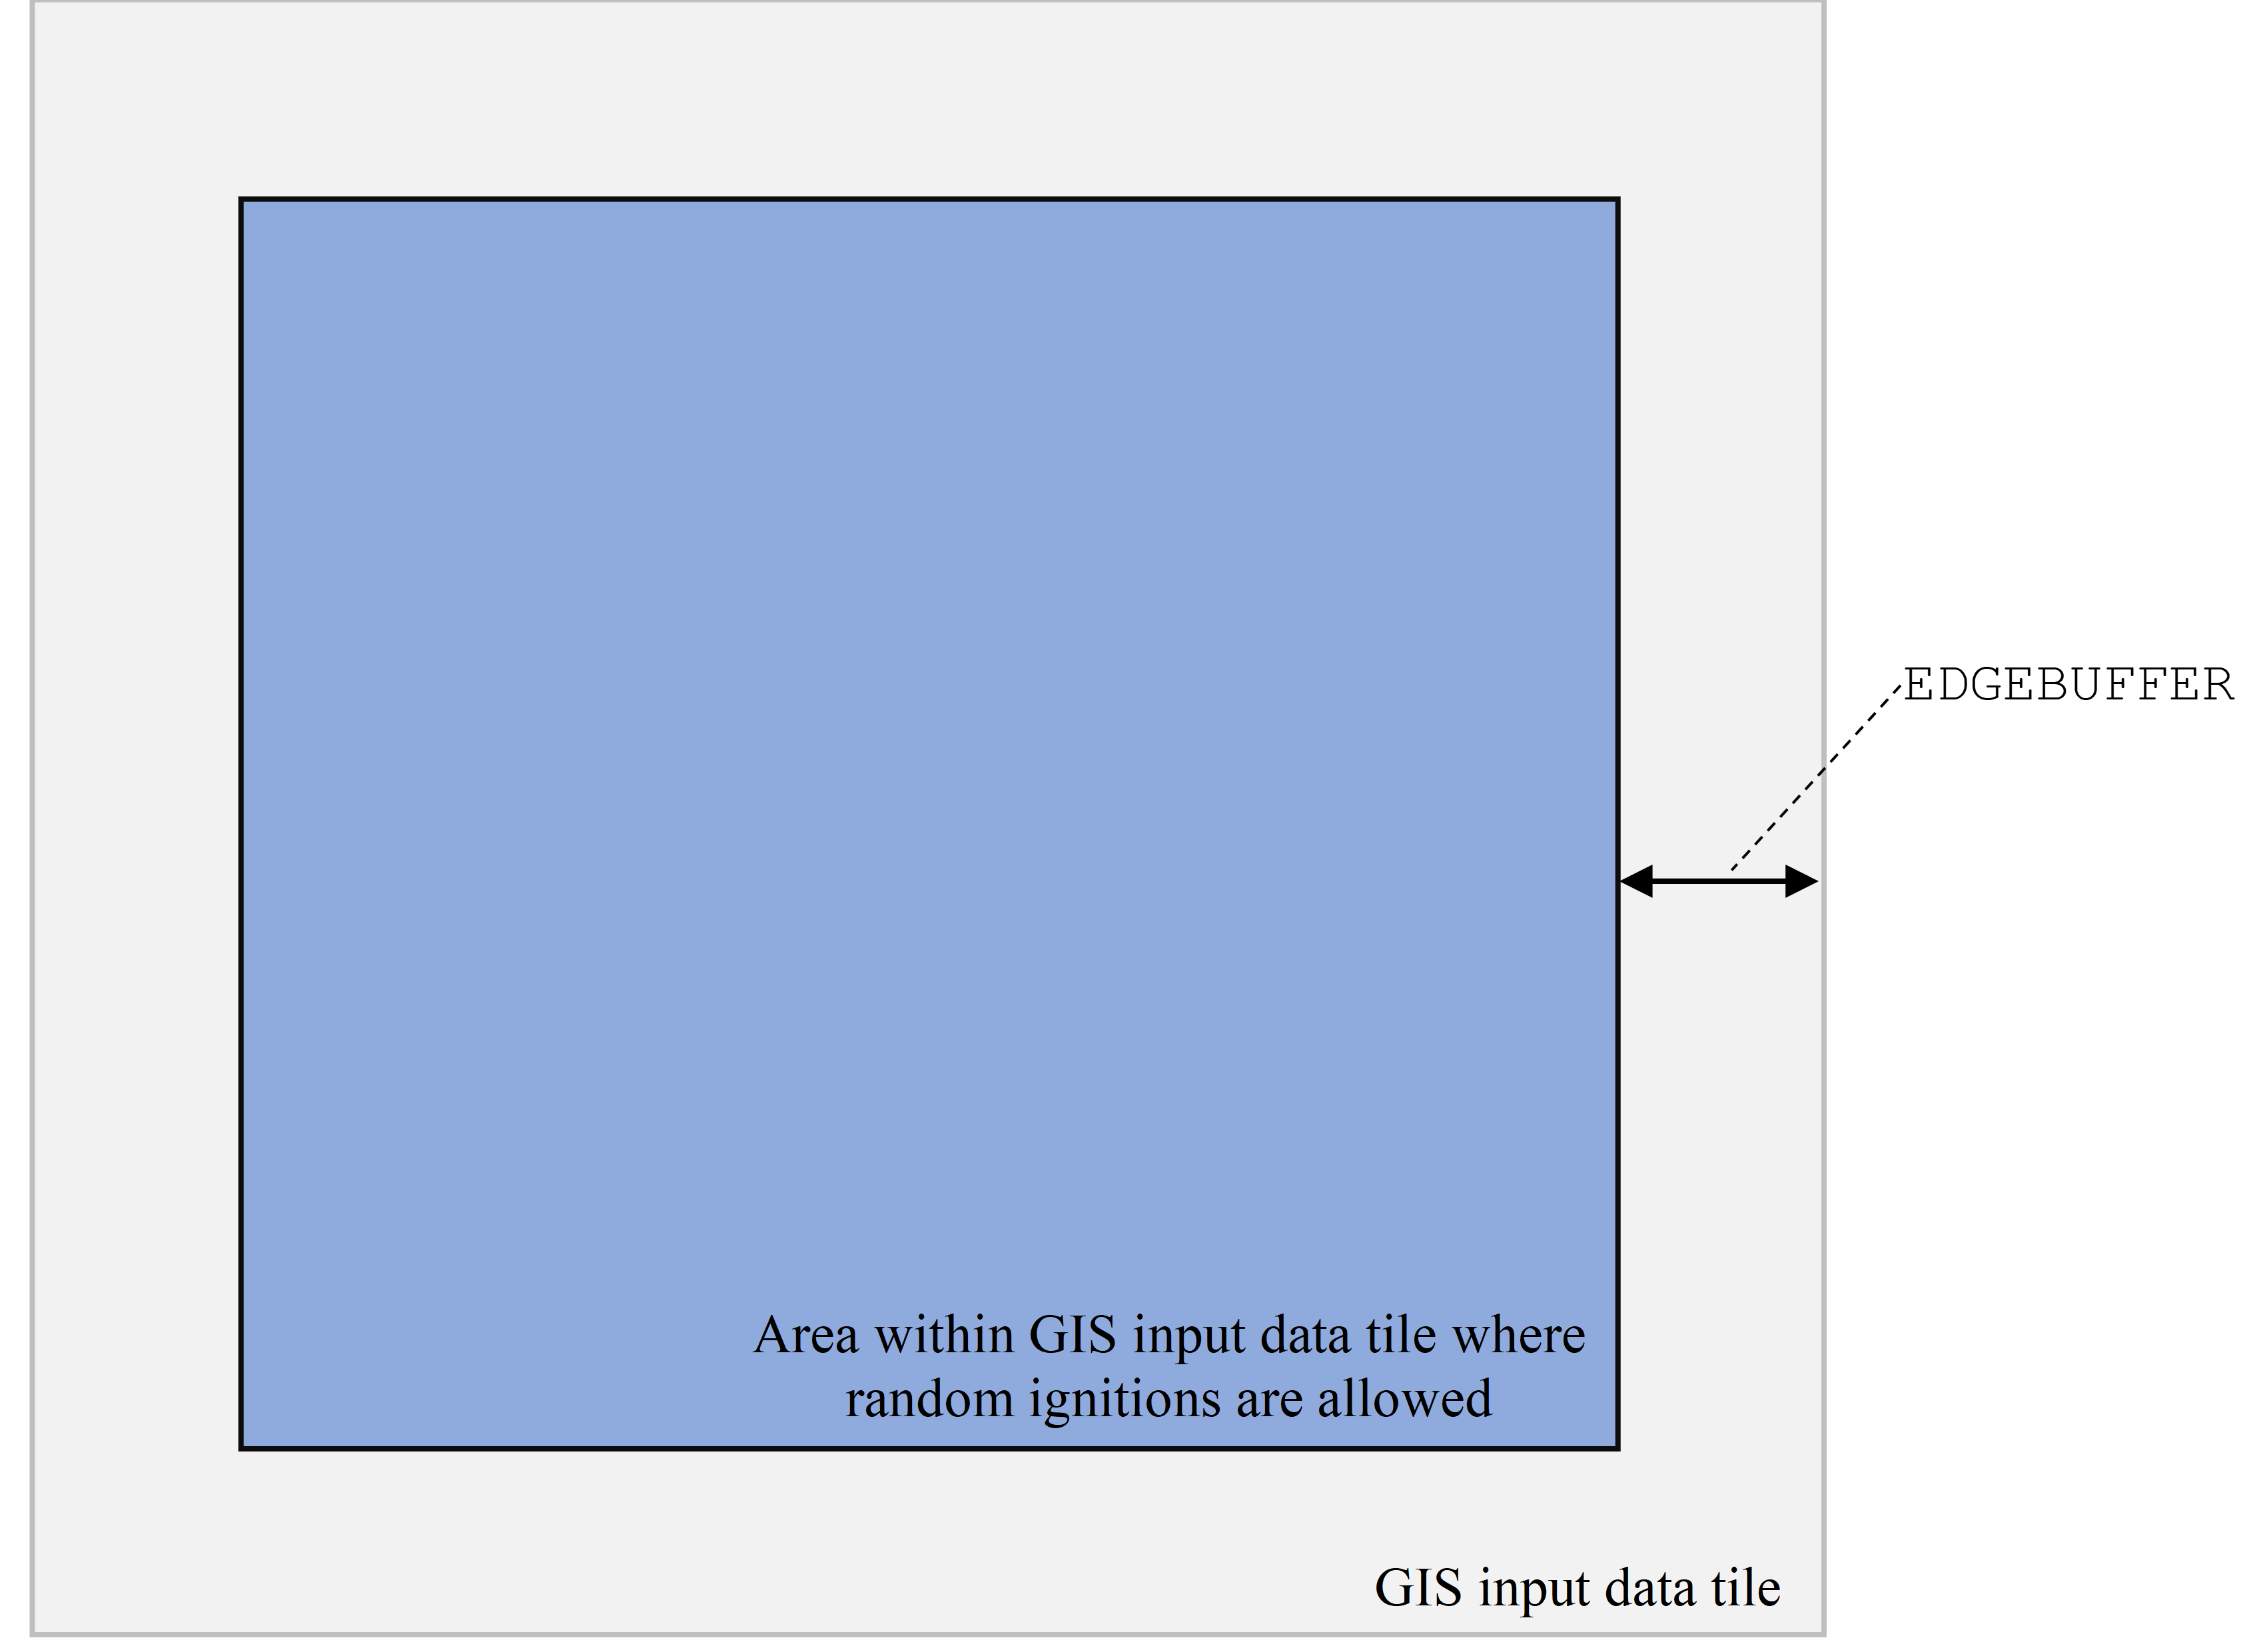
\includegraphics[width=0.7\linewidth]{figs/random_ignition_buffer.png}
    \caption{A graphical display of EDGEBUFFER.}
    \label{fig:edgebuffer}
\end{figure}

Random ignition location may also be constrained by an ignition mask raster. To do this, set USE\_IGNITION\_MASK = .TRUE. and specify IGNITION\_MASK\_FILENAME on the \&INPUTS line. This directs ELMFIRE to read a Float32 raster named IGNITION\_MASK\_FILENAME.tif from the FUELS\_AND\_TOPOGRAPHY\_DIRECTORY. You can also build an ignition mask within ELMFIRE by automatically excluding all nonburnable cells, by setting ADD\_TO\_IGNITION\_MASK = .TRUE.. If the user wants to include nonburnable pixels to be potential ignition spots, then set ALLOW\_NONBURNABLE\_PIXEL\_IGNITION to .TRUE. in the \&SIMULATOR namelist.

Distribution of ignitions across the landscape is controlled by the parameter RANDOM\_IGNITIONS\_TYPE:

\begin{itemize}
    \item RANDOM\_IGNITIONS\_TYPE=1 (default): Ignitions are spatially distributed uniformly across the landscape in any pixels where the ignition mask raster is greater than zero. This is useful for modeling ignitions originating from powerlines or roads, for example.
    \item RANDOM\_IGNITIONS\_TYPE=2: Ignitions are spatially distributed across the landscape at a density that is proportional to the ignition mask raster. This is useful for burn probability modeling where some locations across the landscape have higher ignition probabilities than other locations. A global IGNITION\_MASK\_SCALE\_FACTOR can be set to upscale or downscale the mask for calibration or optimization.
\end{itemize}

The number of randomly-generated ignition points can be specified in two ways:

By directly specifying NUM\_ENSEMBLE\_MEMBERS, or

By specifying PERCENT\_OF\_PIXELS\_TO\_IGNITE and setting NUM\_ENSEMBLE\_MEMBERS to a value less than 0.

In the first case, ELMFIRE will randomly generate NUM\_ENSEMBLE\_MEMBERS ignition locations in the allowable ignition area as defined by EDGEBUFFER (and, if USE\_IGNITION\_MASK = .TRUE., the user-specified ignition mask raster as well). In the second case, ELMFIRE will count all pixels within the allowable ignition area and randomly ignite the user-specified percent of those pixels. In some cases, a pixel may be selected more than once to be ignited. This can be disabled by setting ALLOW\_MULTIPLE\_IGNITIONS\_AT\_A\_PIXEL = .FALSE..

Ignitions can also be set manually though a csv file with coordinates of ignitions. Setting CSV\_FIXED\_IGNITION\_LOCATIONS = .TRUE. will instruct ELMFIRE to look for a file called IGNITIONS\_CSV\_FILENAME.csv within the FUELS\_AND\_TOPOGRAPHY\_DIRECTORY folder. 

\subsection{Randomized weather streams}
\label{randomized_weather}

In the example discussed in Randomized ignition locations, ignition locations are selected randomly and a single weather stream (hindcast or forecast) is provided as input to those simulations. Often, as part of a climatological fire risk analysis, it is desirable to simulate wind and weather conditions under a range of historical (or forecasted) wind and weather conditions. This can be accomplished in ELMFIRE using stacked/multiband weather/meteorology rasters.

The manner in which these rasters are used is controlled by the parameters NUM\_METEOROLOGY\_TIMES, METEOROLOGY\_BAND\_START, METEOROLOGY\_BAND\_STOP, and METEOROLOGY\_BAND\_SKIP\_INTERVAL. This is perhaps best illustrated by an example. Assume that numerical weather prediction has been used to generate 100 24-hour “blocks” of historical wind/weather data at hourly intervals that will be provided as input to a Monte Carlo analysis. The goal is to simulate 24-hours of fire spread, for each of these 24-hour blocks. However, these 24-hour blocks are not temporally contiguous, meaning the first 24-hour block could be from August 1983 and the next 24-hour block could be from October 2012, and so on.

Each 24-hour block consists of 25 bands since Band 1 is $t = 0$ and Band 25 is $t = 24$ hours. Therefore, each meteorology raster would contain 2,500 separate bands (100 blocks $\times$ 25 bands per block). Since ELMFIRE needs 25 bands of wind/weather data to drive each 24-hour simulation, we would set METEOROLOGY\_BAND\_START=1, METEOROLOGY\_BAND\_STOP=2476, and METEOROLOGY\_BAND\_SKIP\_INTERVAL=25. This tells ELMFIRE to use every 25th band as the starting band for a 24-hour simulation and ensures that each 24-hour simulation starts with Band 1, 26, 51, and so on until the final 24-hour block is reached at meteorology band 2476.

If, instead, the 100 24-hour blocks were temporally contiguous (for example, a continuous hindcast from mid-July through the end of October) and the purpose of the Monte Carlo analysis is to ignite fires every 3 hours and model their spread, we would set METEOROLOGY\_BAND\_SKIP\_INTERVAL=4.

The output of each weather band range will be saved as a separate raster file, with the band number appended at the end. This number is restricted to 3 digits, but 4 can be used by adding USE\_FOUR\_DIGITS\_IN\_IWX\_BAND = .TRUE..

\subsection{Spatial and temporal perturbations of input rasters}
\label{spatial_temporal_pertrubations}

All inputs are subject to inherent uncertainty. To address this uncertainty, input rasters may be perturbed stochastically from their baseline values in a Monte Carlo analysis. Currently, the following rasters may be perturbed:

\begin{itemize}
    \item ADJ: Spread rate adjustment factor (-)
    \item CBD: Canopy bulk density ($kg/m^3$)
    \item CBH: Canopy base height (m)
    \item CC: Canopy cover (-)
    \item CH: Canopy height (m)
    \item FMC: Foliar moisture content (-)
    \item M1: 1-hour fuel moisture (-)
    \item M10: 10-hour fuel moisture (-)
    \item M100: 100-hour fuel moisture (-)
    \item MLH: Live herbaceous fuel moisture (-)
    \item MLW: Live woody fuel moisture (-)
    \item WAF: Wind adjustment factor (-)
    \item WD: Wind direction (deg)
    \item WS: Wind speed (mph)
\end{itemize}

Parameters controlling stochastic perturbations of input rasters are specified in the \&MONTE\_CARLO namelist group. A random sampling procedure is implemented such that the spatial perturbation to be applied to a given input raster sampled from a probability density function (pdf). Currently, only a uniform pdf is implemented (PDF\_TYPE(:) = 'UNIFORM') although this will eventually be generalized to additional distributions such as Gaussian and lognormal. The keyword NUM\_RASTERS\_TO\_PERTURB prescribes the number of input rasters to be perturbed and the keyword RASTER\_TO\_PERTURB(:) is a string corresponding to one of the raster names in the bulleted list above (ADJ, CBD, etc.). As an example, consider the following lines:
\begin{verbatim}
NUM_RASTERS_TO_PERTURB   = 1
RASTER_TO_PERTUB(1)      = 'ADJ'
SPATIAL_PERTURBATION(1)  = 'GLOBAL'
TEMPORAL_PERTURBATION(1) = 'STATIC'
PDF_TYPE(1)              = 'UNIFORM'
PDF_LOWER_LIMIT(1)       = -0.10
PDF_UPPER_LIMIT(1)       = 0.10
\end{verbatim}

These lines specify that a randomly selected value between -0.1 and 0.1 should be added to the spread rate adjustment factor(ADJ). This perturbation will be applied globally to all pixels (SPATIAL\_PERTURBATION = 'GLOBAL') and is temporally invariant for the duration of the simulation (TEMPORAL\_PERTURBATION = 'STATIC'). Rather than applying such perturbations globally to all pixels, different perturbations can be applied to different pixels by setting SPATIAL\_PERTURBATION = 'PIXEL'. Some raster inputs, such as wind speed and direction, are multi-band rasters that vary temporally. Different perturbations may be applied at each time by setting TEMPORAL\_PERTURBATION = 'DYNAMIC'. Normally, this would only be done for wind speed and direction.

The number of ensemble members in the Monte Carlo analysis should be specified using the keyword NUM\_ENSEMBLE\_MEMBERS (\&MONTE\_CARLO namelist group). However, when using randomly-placed ignitions it may instead be preferable to specify the total number of ensemble members by specifying the percentage of pixels within the computational domain and possibly within a user-specified ignition mask to ignite. This is described in Randomized ignition locations.

\subsection{Randomized wind fluctuation intensities}
\label{randomized_wind_fluctuation}

Wind fluctuations are implemented by changing PERTURB\_WIND\_DIRECTION\_FLUCTUATION\_INTENSITY and PERTURB\_WIND\_SPEED\_FLUCTUATION\_INTENSITY to .TRUE. respectively. The keywords that control these fluctuations are WIND\_SPEED\_FLUCTUATION\_INTENSITY and WIND\_DIRECTION\_FLUCTUATION\_INTENSITY. These values can be randomized by setting the following four parameters (in the \&MONTE\_CARLO namelist group):

\begin{itemize}
    \item WIND\_DIRECTION\_FLUCTUATION\_INTENSITY\_MIN: Minimum wind direction fluctuation intensity value
    \item WIND\_DIRECTION\_FLUCTUATION\_INTENSITY\_MAX: Maximum wind direction fluctuation intensity value
    \item WIND\_SPEED\_FLUCTUATION\_INTENSITY\_MIN: Minimum wind speed fluctuation intensity value
    \item WIND\_SPEED\_FLUCTUATION\_INTENSITY\_MAX: Maximum wind speed fluctuation intensity value
\end{itemize}

The wind fluctuation intensities are then randomly generated according to a uniform probability density function, with the upper and lower values specified by the above four parameters.

\subsection{Outputs}
\label{monte_carlo_outputs}

Several outputs are specific to Monte Carlo analyses. Often, when conducting a Monte Carlo analysis with randomly distributed ignitions, it is informative to view spatial burn probabilities, defined as the fraction of simulations in which a given pixel burned. To enable this calculation (which adds some computational and network overhead), set CALCULATE\_TIMES\_BURNED = .TRUE. in the \&OUTPUTS namelist group. 

This instructs ELMFIRE to aggregate all simulated fire perimeters and calculate the burn probability across all runs and write the results to disk (in a file called burn\_probability.tif). The output raster has three bands. The first is the conventional burn probability. The second is passive crown fire burn probability, meaning the fraction of times in which a pixel burned as passive crown fire. The third band is active crown fire burn probability.

\section{Building Fire Spread}
\label{building_spread}

ELMFIRE contains an experimental building fire spread model based on the work of Purnomo et al (2024). Most Rothermel-based models consider built-up areas nonburnable, as urban conflagrations were not an issue when the model was developed. As such, neither the spread mechanisms nor any 'building' fuel models were developed. This model attemts to work with the same principles as the Rothermel model, in using elliptical fire spread from a discretized point source to spread the fire. More details can be found in the mathematical section. 

It can be turned on through USE\_BLDG\_SPREAD\_MODEL = .TRUE.. The input parameters can either be provided as constants for the entire simulation domain (by setting USE\_CONSTANT\_BLDG\_SPREAD\_MODEL\_PARAMS = .TRUE. (set .TRUE. as default. The BUILDING\_FUEL\_MODEL\_FILE needs to be specified. The option BLDG\_SPREAD\_MODEL\_TYPE can be set to choose between the Hamada model (1) and the UCB-UMD WU-E model (2). 

The universal input parameters can be set:

\begin{itemize}
    \item BLDG\_AREA\_CONSTANT (building area footprint, $m^2$)
    \item BLDG\_SEPARATION\_DIST\_CONSTANT (building separation distance, m)
    \item BLDG\_NONBURNABLE\_FRAC\_CONSTANT
    \item BLDG\_FOOTPRINT\_FRAC\_CONSTANT
    \item BLDG\_FUEL\_MODEL\_CONSTANT (fuel model number)
\end{itemize}

The equivalent raster inputs, specified in \&INPUTS are:

\begin{itemize}
    \item BLDG\_AREA\_FILENAME
    \item BLDG\_SEPARATION\_DIST\_FILENAME
    \item BLDG\_NONBURNABLE\_FRAC\_FILENAME
    \item BLDG\_FOOTPRINT\_FRAC\_FILENAME
    \item BLDG\_FUEL\_MODEL\_FILENAME
\end{itemize}

Extra outputs can be specified with the building spread model. Turning ESTIMATE\_URAN\_LOSSES = .TRUE. in the \&OUTPUTS namespace will include the results of the building fire spread to the affected population and surface fire area statistics.

\section{Suppression}
\label{suppression}

ELMFIRE can model the effects of suppression efforts on the fire front. While it cannot model individual firefighting action on the landscape, it can estimate the effectiveness of an initial attack, and the containment progress of an extended firefighting attack.

Initial attack can be activated through the switch ENABLE\_INITIAL\_ATTACK in the \&SUPPRESSION namelist. Then the time of the attack can be specified through INITIAL\_ATTACK\_TIME in seconds. Depending on the fire area and average fireline intensity, the initial attack then has a probability of successfully containing the fire. If the fire is successfully contained then the simulation stops.

Extended attack can be activated through an example script below:

\begin{verbatim}
&INPUTS
...
SDI_FILENAME               = 'sdi'
...

&SUPPRESSION
ENABLE_EXTENDED_ATTACK     = .TRUE.
DT_EXTENDED_ATTACK         = 3600
AREA_NO_CONTAINMENT_CHANGE = 10000
MAX_CONTAINMENT_PER_DAY    = 100
SDI_FACTOR                 = 1
USE_SDI                    = .TRUE.
USE_SDI_LOG_FUNCTION       = .TRUE.
B_SDI                      = 1
\end{verbatim}

In the code snippet above, the option input of Suppression Difficulty Index (SDI) is used, to differentiate cells with high SDI (~1) or low SDI (~0). SDI\_FACTOR can be used to scale all SDI values for optimisation or calibration. 

The critical part of calculating containment is the containment change per DT\_EXTENDED\_ATTACK. Every such timestep, the change in containment is calculated by comparing the change in wildfire area and the AREA\_NO\_CONTAINMENT\_CHANGE. Based on these two values, the SDI, the MAX\-CONTAINMENT\_PER\_DAY, (100 means that 100\% of the possible containment change will be applied), and B\_SDI (a scaling factor). The effect of area change to the containment change is linear as standard but can be changed to logarithmic through USE\_SDI\_LOG\_FUNCTION. The area comparison mentioned above takes SDI into account (meaning the change of fire area is scaled by the relative suppression difficulty of the new cells). If SDI data are not available for an area, USE\_SDI can be set to .FALSE., and a factor of 1 will be used throughout the simulation. 

\section{Fire Potential Mode}
\label{fire_potential}

So far, ELMFIRE has been set to estimate the fire propagation based on some starting conditions and (potentially) transient weather. This is similar to the function of FARSITE. ELMFIRE is also capable of estimating the fire risk of an area at a given weather, much like the FLAMMAP program. This behavior is controlled through the MODE variable. 

The modes that ELMFIRE has are:

\begin{itemize}
    \item MODE = 1: The standard ELMFIRE spread model, with (potentially) transient weather, ignitions, firebrands, level set propagation. 
    \item MODE = 2: Fire potential mode. No ignitions are provided, instead ELMFIRE calculated the maximum rate of spread and potential crown fire activity for all cells of the domain, for each weather band. 
    \item MODE = 3: Both output types from above. 
\end{itemize}

\section{Assets at Risk}
\label{assets_at_risk}

An important part of quantifying fire risk is assessing potential impacts to assets at risk. ELMFIRE is currently capable of quantifying impacts to three assets at risk. Since some of the most relevant assets at risk are population, real estate/structures, and land/timber, the keywords that are used to specify assets at risk in the \&INPUTS namelist group are hardcoded as REAL\_ESTATE, POPULATION\_DENSITY, and LAND\_VALUE although each of these is treated identically. Since other assets at risk may be relevant (cultural resources, sensitive habitat, watershed, etc.), the total number of assets at risk eventually will be expanded. However, for the time being, assets at risk are specified as follows:

\begin{itemize}
    \item Land value: Set USE\_LAND\_VALUE = .TRUE. and specify the land value filename via LAND\_VALUE\_FILENAME
    \item Real estate value: Set USE\_REAL\_ESTATE\_VALUE = .TRUE. and specify the real estate value filename via REAL\_ESTATE\_VALUE\_FILENAME
    \item Population density: Set USE\_POPULATION\_DENSITY = .TRUE. and specify the population density filename via POPULATION\_DENSITY\_FILENAME
\end{itemize}

Note that assets at risk are read in from the FUELS\_AND\_TOPOGRAPHY directory. Additionally, all assets at risk should be Float32 GeoTiff rasters. Units should be quantity per acre, e.g. structures per acre, population per acre, \$ per acre, etc.

If assets at risk rasters are provided as input, ELMFIRE will sum total impacts by integrating fire area over asset at risk density and report this in the fire\_size\_stats.csv output file. ELMFIRE will also create impact rasters affected\_land\_value.tif, affected\_real\_estate\_value.tif, and affected\_population.tif.

\section{Pyrome Calibration}
\label{calibration}

Large areas of the landscape can be categorised or delineated based on their historic fire conditions, or the way that wildfires historically spread and behave. Such areas are called Pyromes, and outline areas of similar fire behavior beyond having similar fuels, weather patterns or topography. Such delineations require expert judgement or knowledge of the local fire landscape, though an initial delineation of the continental United States, along with guides on how they can be generated, can be found in Short et al. 

If the simulation area contains multiple pyromes, the fire behaviour of each area can be adjusted. Pyrome adjustment can be activated through USE\_PYROMES = .TRUE. in the \&SIMULATOR namelist. A raster named PYROMES\_FILENAME.tif can be specified in the \&INPUTS namelist. Each point in that raster is assigned an integer, specifying which pyrome it belongs to. Subsequent Pyrome files belong to the \&CALIBRATION namelist can be specified to make adjustments to various parameters depending on which pyrome they belong to. As an example, below is a sample file which contains different adjustment factors, ADJUSTMENT\_FACTORS\_FILENAME (which requires ADJUSTMENT\_FACTORS\_BY\_PYROME = .TRUE. to be used):

\begin{verbatim}
   108 121 162 163 181 202
1  1.0 1.1 1.1 0.9 1.0 0.8
2  1.1 1.0 0.9 1.0 1.2 1.0
3  1.2 1.0 1.0 1.1 1.1 0.9
4  1.0 0.8 1.1 0.9 1.0 0.8
\end{verbatim}

In the case of ADJUSTMENT\_FACTORS\_FILENAME, each of these values adjusts the predicted surface and crown fire rates of spread. For example, within pyrome 3, surface and crown fire rate of spread will be multiplied by 1.2 for cells with fuel model 108, 1.0 for fuel model 121 and so on.  

If CALIBRATION\_CONSTANTS\_BY\_PYROME is set to .TRUE., and accompanying CALIBRATION\_CONSTANTS\_FILENAME file should be provided, with the structure:

\begin{verbatim}
   InitialAttackTime BSDI MAXCPERDAY AREANCCHANGE SIMDURATION IGNDENSITYADJ
1  3600              0.9  100        10000        16000       0.8
2  3600              1.0  90         8500         12000       1.0
3  3600              1.0  100        10000        16000       0.9
4  1800              0.9  100        10000        14000       0.8
\end{verbatim}

The spaces between the values are just added here to illustrate which column they correspond to, they are not necessary. The columns are, in order, suppression initial attack time, adjustment factor $B_SDI$, max containment per day, area of no containment change, ELMFIRE simulation duration and ignition density (probability) adjustment. See the Suppression section for more details on the first four parameters, and the monte carlo (ignition) section for the latter two. 

For long-term monte carlo simulations, another way to set the total simulation time is by providing probability density functions to individual day durations. By setting DURATION\_PDF\_BY\_PYROME = .TRUE., an input file DURATION\_PDF\_FILENAME can be specified:

\begin{verbatim}
   1     2     3   ... 364   355 
1  0.000 0.001 0.050   0.000 0.000
2  0.000 0.001 0.001   0.010 0.000
3  0.000 0.001 0.100   0.000 0.000
...
\end{verbatim}

Each value denotes the probability that the duration of the simulation will be equal to that day duration. A hard limit of DURATION\_MAX\_DAYS is set, so no simulation can be longer. 


\section{Smoke}

ELMFIRE has placeholder values for a future smoke submodel. This submodel has not yet been implemented, and as such this section of the guide has been left as a placeholder for future versions.


\section{Process Flowchart}

ELMFIRE Workflow:
\begin{enumerate}
    \item Setup variables
    \item Setup MPI
    \item Read and check input file
    \item Set randomizer seed
    \item Calculate sunrise and sunset times
    \item Calculate and save lookup tables (for easy/fast access)
    \item Read headers of fuels \& topography
    \item Read weather, fuels \& topography raster data
    \item Determine number of cases to run
    \item Rotate wind if GRID\_DECLINATION
    \item If pyromes are used, parse adjustment factors
    \item Remap the input grids (coarse) to the simulation cellsize (fine)
    \item Allocate additional intermediate rasters (outputs, intermediate rasters etc.)
    \item (if Random Ignitions) Determine ignition locations
    \item Allocate output rasters
    \item If in fire potential mode (MODE = 2 or 3)
    \begin{enumerate}
        \item Initialize spread output rasters
        \item Keep track of all burnable cells (burnable fuel types and outside of Edgebuffer range) 
        \item For each weather band:
        \begin{enumerate}
            \item Calculate surface and crown spread rates
            \item Check surface flame length, if high enough then keep max spread of surface and crown.
            \item Output spread raster values
        \end{enumerate}
    \end{enumerate}
    \item If in fire spread mode (MODE = 1 or 3)
    \begin{enumerate}
        \item (ensemble monte carlo) initialize random parameters and pretrubations.
        \item For each scenario call level set propagation algorithm.
        \item Accumulate ensemble statistics
        \item Run postprocessing for advanced outputs
    \end{enumerate}
    \item Shutdown
\end{enumerate}

Main level set propagation algorithm:
\begin{enumerate}
    \item Determine simulation stop time
    \item If its the first time level set is called:
    \begin{enumerate}
        \item Allocate intermediate rasters
        \item Determine output time interval
        \item Allocate output rasters
        \item Set pointer addresses
    \end{enumerate}
    \item If random ignitions are on:
    \begin{enumerate}
        \item Set ignition location
        \item Adjust simulation time and suppression parameters through Pyrome
        \item Exclude and set outputs if nonburnable cell is selected for ignition
    \end{enumerate}
    \item Check that weather band exists for this time step
    \item Initialize weather, suppression, point list variables
    \item If random ignitions are not enabled:
    \begin{enumerate}
        \item Check each landscape point for $\phi < 0$, set as burning, and set initial weather parameters
        \item Calculate surface and crown rates of spread for all points currently burning
        \item Calculate front normal vectors, calculate X and Y ROS components
        \item Check for eligible fire spread cells within fire front BANDTHICKNESS
    \end{enumerate}
    \item Start the main loop:
    \begin{enumerate}
        \item If applicable, calculate overnight adjustment factor time span
        \item If random ignitions are on, set $\phi$ of ignition point to zero and save potential spread points.
        \item If multiple ignitions are specified in the input, check if any new ignitions apply.
        \item Interpolate current weather values
        \item Apply wind fluctuations
        \item Calculate surface spread rate
        \item Calculate crown spread rate
        \item Calculate components of normal vectors of fire front
        \item Calculate Ux and Uy velocity components
        \item Calculate new time step with CFL and Flux limiter
        \item Integrate level set equations with Runge Kutta 2nd order
        \item Update burning point values and statistics
        \item If enabled, save binary outputs
        \item If enabled, calculate new spot fire locations
        \item If UMD spotting is enabled, calculate physical parameters and run spotting model.
        \item Calculate and clear extinguished embers (separate processes for eulerian and lagrangian)
        \item Calculate interpolated weather values for newly-included cells
        \item Calculate surface and crown spread rates for new cells
        \item If applicable, calculate initial attach probability
        \item Stop simulation if less than two points are burning, or if a max acreage criterion is reached.
        \item If applicable, append acreage timings statistics
        \item Calculate extended attack containment
        \item Dump main outputs
    \end{enumerate}
    \item Process and output timed location data (does not apply to newer versions).
    \item Calculate and output fire size statistics
    \item If applicable, dump binary outputs
    \item If applicable, dump ember count bin measurements.
\end{enumerate}



